
\documentclass[12pt, a4paper]{report}
\usepackage{epsfig}
\usepackage{subfigure}
%\usepackage{amscd}
\usepackage{amssymb}
\usepackage{graphicx}
%\usepackage{amscd}
\usepackage{amssymb}
\usepackage{subfiles}
\usepackage{framed}
\usepackage{subfiles}
\usepackage{amsthm, amsmath}
\usepackage{amsbsy}
\usepackage{framed}
\usepackage[usenames]{color}
\usepackage{listings}
\lstset{% general command to set parameter(s)
basicstyle=\small, % print whole listing small
keywordstyle=\color{red}\itshape,
% underlined bold black keywords
commentstyle=\color{blue}, % white comments
stringstyle=\ttfamily, % typewriter type for strings
showstringspaces=false,
numbers=left, numberstyle=\tiny, stepnumber=1, numbersep=5pt, %
frame=shadowbox,
rulesepcolor=\color{black},
,columns=fullflexible
} %
%\usepackage[dvips]{graphicx}
\usepackage{natbib}
\bibliographystyle{chicago}
\usepackage{vmargin}
% left top textwidth textheight headheight
% headsep footheight footskip
\setmargins{3.0cm}{2.5cm}{15.5 cm}{22cm}{0.5cm}{0cm}{1cm}{1cm}
\renewcommand{\baselinestretch}{1.5}
\pagenumbering{arabic}
\theoremstyle{plain}
\newtheorem{theorem}{Theorem}[section]
\newtheorem{corollary}[theorem]{Corollary}
\newtheorem{ill}[theorem]{Example}
\newtheorem{lemma}[theorem]{Lemma}
\newtheorem{proposition}[theorem]{Proposition}
\newtheorem{conjecture}[theorem]{Conjecture}
\newtheorem{axiom}{Axiom}
\theoremstyle{definition}
\newtheorem{definition}{Definition}[section]
\newtheorem{notation}{Notation}
\theoremstyle{remark}
\newtheorem{remark}{Remark}[section]
\newtheorem{example}{Example}[section]
\renewcommand{\thenotation}{}
\renewcommand{\thetable}{\thesection.\arabic{table}}
\renewcommand{\thefigure}{\thesection.\arabic{figure}}
\title{Research notes: linear mixed effects models}
\author{ } \date{ }


\begin{document}
\author{Kevin O'Brien}
\title{Mixed Models for Method Comparison Studies}
\tableofcontents

%----------------------------------------------------------------------------------------%
\newpage






\chapter{Other Material}
%========================================================================== %

\section{Implementation in R}
To implement an LME model in \texttt{R}, the \texttt{nlme} package is used. This package is loaded into the \texttt{R} environment using the library command, (i.e.\ \texttt{library(nlme)}). The \texttt{lme} command is used to fit LME models. The first two arguments to the \texttt{lme} function specify the fixed effect component of the model, and the data set to which the model is to be fitted. The first candidate model (`MCS1') fits an LME model on the data set `dat'. The variable `method' is assigned as the fixed effect, with the response variable `BP' (i.e.\ blood pressure).

The third argument contain the random effects component of the formulation, describing the random effects, and their grouping structure. The \texttt{nlme} package provides a set of positive-definite matrices , the \texttt{pdMat} class, that can be used to specify a structure for the between-subject variance-covariance matrix for the random effects. For Roy's methodology, we will use the \texttt{pdSymm} and \texttt{pdCompSymm} to specify a symmetric structure and a compound symmetry structure respectively. A full discussion of these structures can be found in \citet[pg. 158]{PB}.

Similarly a variety of structures for the with-subject variance-covariance matrix can be implemented using \texttt{nlme}. To implement a particular matrix structure, one must specify both a variance function and correlation structure accordingly. Variance functions are used to model the variance structure of the within-subject errors. \texttt{varIdent} is a variance function object used to allow different variances according to the levels of a classification factor in the data. A compound symmetry structure is implemented using the \texttt{corCompSymm} class, while the symmetric form is specified by \texttt{corSymm} class. Finally, the estimation methods is specified as ``ML" or ``REML".
\newpage
The first of Roy's candidate model can be implemented using the following code;\\

\begin{framed}
	\begin{verbatim}
	MCS1 = lme(BP ~ method-1, data = dat,
	random =  list(subject=pdSymm(~ method-1)),
	weights=varIdent(form=~1|method),
	correlation = corSymm(form=~1 | subject/obs), method="ML")
	\end{verbatim}
\end{framed}

For the blood pressure data used in \citet{ARoy2009}, all four candidate models are implemented by slight variations of this piece of code, specifying either \texttt{pdSymm} or \texttt{pdCompSymm} in the second line, and either \texttt{corSymm} or \texttt{corCompSymm} in the fourth line.
For example, the second candidate model `MCS2' is implemented with the same code as MCS1, except for the term \texttt{pdCompSymm} in the second line, rather than \texttt{pdSymm}.



\begin{framed}
	\begin{verbatim}
	MCS2 = lme(BP ~ method-1, data = dat,
	random = list(subject=pdCompSymm(~ method-1)),
	weights = varIdent(form=~1|method),
	correlation = corSymm(form=~1 | subject/obs), method="ML")
	\end{verbatim}
\end{framed}
\vspace{1cm}
Using this \texttt{R} implementation for other data sets requires that the data set is structured appropriately (i.e.\ each case of observation records the index, response, method and replicate). Once formatted properly, implementation is simply a case of re-writing the first line of code, and computing the four candidate models accordingly.
\newpage
To perform a likelihood ratio test for two candidate models, simply use the \texttt{anova} command with the names of the candidate models as arguments. The following piece of code implement the first of Roy's variability tests.
\\
\begin{framed}
	\begin{verbatim}
	> anova(MCS1,MCS2)
	Model df    AIC    BIC  logLik   Test L.Ratio p-value
	MCS1     1  8 4077.5 4111.3 -2030.7
	MCS2     2  7 4075.6 4105.3 -2030.8 1 vs 2 0.15291  0.6958
	>
	\end{verbatim}
\end{framed}
\vspace{1cm}
The fixed effects estimates are the same for all four candidate models. The inter-method bias can be easily determined by inspecting a summary of any model. The summary presents estimates for all of the important parameters, but not the complete variance-covariance matrices (although some simple \texttt{R} functions can be written to overcome this). The variance estimates for the random effects for MCS2 is presented below.
\\
\begin{framed}
	\begin{verbatim}
	Random effects:
	Formula: ~method - 1 | subject
	Structure: Compound Symmetry
	StdDev Corr
	methodJ  30.765
	methodS  30.765 0.829
	Residual  6.115
	\end{verbatim}
\end{framed}
\vspace{1cm}
Similarly, for computing the limits of agreement the standard deviation of the differences is not explicitly given. Again, A simple \texttt{R} function can be written to calculate the limits of agreement directly.

%------------------------------------------------------------------------------------%

\section{Extension of Roy's methodology}
Roy's methodology is constructed to compare two methods in the presence of replicate measurements. Necessarily it is worth examining whether this methodology can be adapted for different circumstances.

An implementation of Roy's methodology, whereby three or more methods are used, is not feasible due to computational restrictions. Specifically there is a failure to reach convergence before the iteration limit is reached. This may be due to the presence of additional variables, causing the problem of non-identifiability. In the case of two variables, it is required to estimate two variance terms and four correlation terms, six in all. For the case of three variabilities, three variance terms must be estimated as well as nine correlation terms, twelve in all. In general for $n$ methods has $2 \times T_{n}$ variance terms, where $T_n$ is the triangular number for $n$, i.e. the addition analogue of the factorial. Hence the computational complexity quite increases substantially for every increase in $n$.

Should an implementation be feasible, further difficulty arises when interpreting the results. The fundamental question is whether two methods have close agreement so as to be interchangeable. When three methods are present in the model, the null hypothesis is that all three methods have the same variability relevant to the respective tests. The outcome of the analysis will either be that all three are interchangeable or that all three are not interchangeable.

The tests would not be informative as to whether any two of those three were interchangeable, or equivalently if one method in particular disagreed with the other two. Indeed it is easier to perform three pair-wise comparisons separately and then to combine the results.



\section{Roy's methodology for single measurements}
Roy's methodology follows from the decomposition for the covariance matrix of the response vector $y_{i}$, as presented in \citet{hamlett}. The decomposition depends on the estimation of correlation terms, which would be absent in the single measurement case. Indeed there can be no within-subject variability if there are no repeated terms for it to describe. There would only be the covariance matrix of the measurements by both methods, which doesn't require the use of LME models. To conlude, simple existing methodologies would be the correct approach where there only one measurements by each method.
Roy's methodology is not suitable for the case of single measurements because it follows from the decomposition for the covariance matrix of the response vector $y_{i}$, as presented in \citet{hamlett}. The decomposition depends on the estimation of correlation terms, which would be absent in the single measurement case. Indeed there can be no within-subject variability if there are no repeated terms for it to describe. There would only be the covariance matrix of the measurements by both methods, which doesn't require the use of LME models. To conclude, simpler existing methodologies, such as Deming regression, would be the correct approach where there only one measurements by each method.

Roy's methodology is not suitable for the case of single measurements because it follows from the decomposition for the covariance matrix of the response vector $y_{i}$, as presented in \citet{hamlett}. The decomposition depends on the estimation of correlation terms, which would be absent in the single measurement case. Indeed there can be no within-subject variability if there are no repeated terms for it to describe. There would only be the covariance matrix of the measurements by both methods, which doesn't require the use of LME models. To conclude, simpler existing methodologies, such as Deming regression, would be the correct approach where there only one measurements by each method.






%-----------------------------------------------------------------------------------%


\section{Correlation}



Bivariate correlation coefficients have been shown to be of
limited use in method comparison studies \citep{BA86}. However,
recently correlation analysis has been developed to cope with
repeated measurements, enhancing their potential usefulness. Roy
incorporates the use of correlation into his methodology.


In addition to the variability tests, Roy advises that it is preferable that a correlation of greater than $0.82$ exist for two methods to be considered interchangeable. However if two methods fulfil all the other conditions for agreement, failure to comply with this one can be overlooked. Indeed Roy demonstrates that placing undue importance to it can lead to incorrect conclusions. \citet{ARoy2009} remarks that current computer implementations only gives overall correlation coefficients, but not their variances. Consequently it is not possible to carry out inferences based on all overall correlation coefficients.

\section{Correlation terms}
\citet{hamlett} demonstrated how the between-subject and within subject variabilities can be expressed in terms of
correlation terms.

\[
\boldsymbol{D} = \left( \begin{array}{cc}
\sigma^2_{A}\rho_{A} & \sigma_{A}\sigma_{b}\rho_{AB}\delta \\
\sigma_{A}\sigma_{b}\rho_{AB}\delta & \sigma^2_{B}\rho_{B}\\

\end{array}\right)
\]

\[
\boldsymbol{\Lambda} = \left(
\begin{array}{cc}
\sigma^2_{A}(1-\rho_{A}) & \sigma_{AB}(1-\delta)  \\
\sigma_{AB}(1-\delta) & \sigma^2_{B}(1-\rho_{B}) \\
\end{array}\right).
\]

$\rho_{A}$ describe the correlations of measurements made by the method $A$ at different times. Similarly $\rho_{B}$ describe the correlation of measurements made by the method $B$ at different times. Correlations among repeated measures within the same method are known as intra-class correlation coefficients. $\rho_{AB}$ describes the correlation of measurements taken at the same same time by both methods. The coefficient $\delta$ is added for when the measurements are taken at different times, and is a constant of less than $1$ for linked replicates. This is based on the assumption that linked replicates measurements taken at the same time would have greater correlation than those taken at different times. For unlinked replicates $\delta$ is simply $1$. \citet{hamlett} provides a useful graphical depiction of the role of each correlation coefficients.

\newpage


%----------------------------------------------------------------------------------------%

\section{Hamlett and Lam}
The methodology proposed by \citet{Roy2009} is largely based on \citet{hamlett}, which in turn follows on from \citet{lam}.

%Lam 99
%In many cases, repeated observation are collected from each subject in sequence  and/or longitudinally.

%Hamlett
%Hamlett re-analyses the data of lam et al to generalize their model to cover other settings not covered by the Lam %method.

Hamlett re-analyses the data of \citet{lam} to generalize their model to cover other settings not covered by the Lam method.

In many cases, repeated observation are collected from each subject in sequence  and/or longitudinally.


\[ y_i = \alpha + \mu_i + \epsilon \]



\section{LaiShiao}


\citet{LaiShiao} advocates the use of LME models to study method comparison problems. The authors analyse a data set typical of method comparison studies using SAS software, with particular use of the \emph{`Proc Mixed'} package. The stated goal of this study is to determine which factor from a specified group of factors is the key contributor to the difference in the two methods.

The study relates to oxygen saturation, the most investigated variable in clinical nursing studies \citep{LaiShiao}. The two method compared are functional saturation (SO2, percent functional oxy-hemoglobin) and fractional saturation (HbO2, percent fractional oxy-hemoglobin), which is considered to be the `gold standard' method of measurement.

\citet{LaiShiao} establishes an LME model for analysing the differences $D_{ijtl}$, where $D_{ijtl}$ is the differences of the measurements (i.e = $SO2_{ijtl}$ - $HbO2_{ijtl}$) for the ith donor at the $j$th level of foetal haemoglobin percent (Fhbperct) and the $t$th repeated measurement by the $l$th practitioner of the experiment.


(\citet{BXC2004} also advocates the use of LME models in comparing methods, but with a different emphasis.)




\section{Lai Shiao}
\citet{LaiShiao} use mixed models to determine the factors that
affect the difference of two methods of measurement using the
conventional formulation of linear mixed effects models.

If the parameter \textbf{b}, and the variance components are not
significantly different from zero, the conclusion that there is no
inter-method bias can be drawn. If the fixed effects component
contains only the intercept, and a simple correlation coefficient
is used, then the estimate of the intercept in the model is the
inter-method bias. Conversely the estimates for the fixed effects
factors can advise the respective influences each factor has on
the differences. It is possible to pre-specify different
correlation structures of the variance components \textbf{G} and
\textbf{R}.


Oxygen saturation is one of the most frequently measured variables
in clinical nursing studies. `Fractional saturation' ($HbO_{2}$)
is considered to be the gold standard method of measurement, with
`functional saturation' ($SO_{2}$) being an alternative method.
The method of examining the causes of differences between these
two methods is applied to a clinical study conducted by
\citet{Shiao}. This experiment was conducted by 8 lab
practitioners on blood samples, with varying levels of
haemoglobin, from two donors. The samples have been in storage for
varying periods ( described by the variable `Bloodage') and are
categorized according to haemoglobin percentages(i.e
$0\%$,$20\%$,$40\%$,$60\%$,$80\%$,$100\%$). There are 625
observations in all.

\citet{LaiShiao} fits two models on this data, with the lab
technicians and the replicate measurements as the random effects
in both models. The first model uses haemoglobin level as a fixed
effects component. For the second model, blood age is added as a
second fixed factor.

\subsubsection{Single fixed effect} The first model fitted by \citet{LaiShiao} takes the
blood level as the sole fixed effect to be analyzed. The following
coefficient estimates are estimated by `Proc Mixed';
\begin{eqnarray}
	\mbox{fixed effects :   } 2.5056 - 0.0263\mbox{Fhbperct}_{ijtl} \\
	(\mbox{p-values :   } = 0.0054, <0.0001, <0.0001)\nonumber\\\nonumber\\
	\mbox{random effects :   } u(\sigma^{2}=3.1826) + e_{ijtl}
	(\sigma^{2}_{e}=0.1525, \rho= 0.6978) \nonumber\\
	(\mbox{p-values :   } = 0.8113, <0.0001, <0.0001)\nonumber
\end{eqnarray}

With the intercept estimate being both non-zero and statistically
significant ($p=0.0054$), this models supports the presence
inter-method bias is $2.5\%$ in favour of $SO_{2}$. Also, the
negative value of the haemoglobin level coefficient indicate that
differences will decrease by $0.0263\%$ for every percentage
increase in the haemoglobin .

In the random effects estimates, the variance due to the
practitioners is $3.1826$, indicating that there is a significant
variation due to technicians ($p=0.0311$) affecting the
differences. The variance for the estimates is given as $0.1525$,
($p<0.0001$).

\subsubsection{Two fixed effects}
Blood age is added as a second fixed factor to the model,
whereupon new estimates are calculated;
\begin{eqnarray}
	\mbox{fixed effects :   } -0.2866 + 0.1072 \mbox{Bloodage}_{ijtl}
	- 0.0264\mbox{Fhbperct}_{ijtl}\nonumber\\
	( \mbox{p-values :   } = 0.8113, <0.0001, <0.0001)\nonumber\\\nonumber\\
	\mbox{random effects :   } u(\sigma^{2}=10.2346) + e_{ijtl}
	(\sigma^{2}_{e}=0.0920, \rho= 0.5577) \nonumber\\
	(\mbox{p-values :   } = 0.0446, <0.0001, <0.0001)
\end{eqnarray}


With this extra fixed effect added to the model, the intercept
term is no longer statistically significant. Therefore, with the
presence of the second fixed factor, the model is no longer
supporting the presence of inter-method bias. Furthermore, the
second coefficient indicates that the blood age of the observation
has a significant bearing on the size of the difference between
both methods ($p <0.0001$). Longer storage times for blood will
lead to higher levels of particular blood factors such as MetHb
and HbCO (due to the breakdown and oxidisation of the
haemoglobin). Increased levels of MetHb and HbCO are concluded to
be the cause of the differences. The coefficient for the
haemoglobin level doesn't differ greatly from the single fixed
factor model, and has a much smaller effect on the differences.
The random effects estimates also indicate significant variation
for the various technicians; $10.2346$ with $p=0.0446$.

\citet{LaiShiao} demonstrates how that linear mixed effects models
can be used to provide greater insight into the cause of the
differences. Naturally the addition of further factors to the
model provides for more insight into the behavior of the data.

\section{Limits of agreement in LME models}

Limits of agreement are used extensively for assessing agreement, because they are intuitive and easy to use.
Necessaire their prevalence in literature has meant that they are now the best known measurement for agreement, and therefore any newer methodology would benefit by making reference to them.

\citet{BXC2008} uses LME models to determine the limits of agreement. Between-subject variation for method $m$ is given by $d^2_{m}$ and within-subject variation is given by $\lambda^2_{m}$.  \citet{BXC2008} remarks that for two methods $A$ and $B$, separate values of $d^2_{A}$ and $d^2_{B}$ cannot be estimated, only their average. Hence the assumption that $d_{x}= d_{y}= d$ is necessary. The between-subject variability $\boldsymbol{D}$ and within-subject variability $\boldsymbol{\Lambda}$ can be presented in matrix form,\[
\boldsymbol{D} = \left(%
\begin{array}{cc}
d^2_{A}& 0 \\
0 & d^2_{B} \\
\end{array}%
\right)=\left(%
\begin{array}{cc}
d^2& 0 \\
0 & d^2\\
\end{array}%
\right),
\hspace{1.5cm}
\boldsymbol{\Lambda} = \left(%
\begin{array}{cc}
\lambda^2_{A}& 0 \\
0 & \lambda^2_{B} \\
\end{array}%
\right).
\]

The variance for method $m$ is $d^2_{m}+\lambda^2_{m}$. Limits of agreement are determined using the standard deviation of the case-wise differences between the sets of measurements by two methods $A$ and $B$, given by
\begin{equation}
	\mbox{var} (y_{A}-y_{B}) = 2d^2 + \lambda^2_{A}+ \lambda^2_{B}.
\end{equation}
Importantly the covariance terms in both variability matrices are zero, and no covariance component is present.

\citet{BXC2008} presents a data set `fat', which is a comparison of measurements of subcutaneous fat
by two observers at the Steno Diabetes Center, Copenhagen. Measurements are in millimeters
(mm). Each person is measured three times by each observer. The observations are considered to be `true' replicates.

A linear mixed effects model is formulated, and implementation through several software packages is demonstrated.
All of the necessary terms are presented in the computer output. The limits of agreement are therefore,
\begin{equation}
	0.0449  \pm 1.96 \times  \sqrt{2 \times 0.0596^2 + 0.0772^2 + 0.0724^2} = (-0.220,  0.309).
\end{equation}

\citet{roy} has demonstrated a methodology whereby $d^2_{A}$ and $d^2_{B}$ can be estimated separately. Also covariance terms are present in both $\boldsymbol{D}$ and $\boldsymbol{\Lambda}$. Using Roy's methodology, the variance of the differences is
\begin{equation}
	\mbox{var} (y_{iA}-y_{iB})= d^2_{A} + \lambda^2_{B} + d^2_{A} + \lambda^2_{B} - 2(d_{AB} + \lambda_{AB})
\end{equation}
All of these terms are given or determinable in computer output.
The limits of agreement can therefore be evaluated using
\begin{equation}
	\bar{y_{A}}-\bar{y_{B}} \pm 1.96 \times \sqrt{ \sigma^2_{A} + \sigma^2_{B}  - 2(\sigma_{AB})}.
\end{equation}

For Carstensen's `fat' data, the limits of agreement computed using Roy's
method are consistent with the estimates given by \citet{BXC2008}; $0.044884  \pm 1.96 \times  0.1373979 = (-0.224,  0.314).$


%------------------------------------------------------------------------------------%

\subsection{Variance Ratios}
Variance Ratios
The approach proposed by Roy deals with the question of agreement, and indeed interchangeability, as developed by Bland and Altman?s corpus of work.  In the view of Dunn, a question relevant to many practitioners is which of the two methods is more precise.

The relationship between precision and the within-item and between-item variability must be established. Roy establishes the equivalence of repeatability and within-item variability, and hence precision.  The method with the smaller within-item variability can be deemed to be the more precise.
A useful approach is to compute the confidence intervals for the ratio of within-item standard deviations (equivalent to the ratio of repeatability coefficients), which can be interpreted in the usual manner.  
In fact, the ratio of within-item standard deviations, with the attendant confidence interval,  can be determined using a single R command: intervals().
Pinheiro and Bates (pg 93-95) give a description of how confidence intervals for the variance components are computed. Furthermore a complete set of confidence intervals can be computed to complement the variance component estimates. 
What is required is the computation of the variance ratios of within-item and between-item standard deviations.  
A na�ve approach would be to compute the variance ratios by relevant F distribution quantiles. However, the question arises as to the appropriate degrees of freedom.
Limits of agreement are easily computable using the LME framework. While we will not be considering this analysis, a demonstration will be provided in the example.


\section{Worked Eamples}

\subsection{LikelihoodRatio Tests}

Conventionally LME models can be tested using Likelihood Ratio Tests, wherein a reference model is compared to a nested model.
\begin{framed}
	\begin{verbatim}
	> Ref.Fit = lme(y ~ meth-1, data = dat,   #Symm , Symm#
	+     random = list(item=pdSymm(~ meth-1)), 
	+     weights=varIdent(form=~1|meth),
	+     correlation = corSymm(form=~1 | item/repl), 
	+     method="ML")
	\end{verbatim}
\end{framed}
Roy(2009) presents two nested models that specify the condition of equality as required, with a third nested model for an additional test. There three formulations share the same structure, and can be specified by making slight alterations of the code for the Reference Model.
Nested Model (Between-Item Variability)
\begin{framed}
	\begin{verbatim}
	> NMB.fit  = lme(y ~ meth-1, data = dat,   #CS , Symm#
	+     random = list(item=pdCompSymm(~ meth-1)),
	+     correlation = corSymm(form=~1 | item/repl), 
	+     method="ML")
	\end{verbatim}
\end{framed}



\begin{framed}
	\begin{verbatim}
	Nested Model (Within ?item Variability)
	> NMW.fit = lme(y ~ meth-1, data = dat,   #Symm , CS# 
	+     random = list(item=pdSymm(~ meth-1)),
	+     weights=varIdent(form=~1|meth), 
	+     correlation = corCompSymm(form=~1 | item/repl), 
	+     method="ML")
	\end{verbatim}
\end{framed}

Nested Model (Overall Variability)
Additionally there is a third nested model, that can be used to test overall variability, substantively a a joint test for between-item and within-item variability. The motivation for including such a test in the suite is not clear, although it does circumvent the need for multiple comparison procedures in certain circumstances, hence providing a simplified procedure for non-statisticians.

\begin{framed}
	\begin{verbatim}
	> NMO.fit = lme(y ~ meth-1, data = dat,   #CS , CS# 
	+     random = list(item=pdCompSymm(~ meth-1)), 
	+     correlation = corCompSymm(form=~1 | item/repl), 
	+     method="ML")
	\end{verbatim}
\end{framed}

ANOVAs  for  Original Fits
The likelihood Ratio test is very simple to implement in R. All that is required it to specify the reference model and the relevant nested mode as arguments to the command anova().
The figure below displays the three tests described by Roy (2009).

\begin{framed}
	\begin{verbatim}
	> testB    = anova(Ref.Fit,NMB.fit)                          # Between-Subject Variabilities
	> testW   = anova(Ref.Fit,NMW.fit)                        # Within-Subject Variabilities
	> testO     = anova(Ref.Fit,NMO.fit)                        # Overall Variabilities
	
	\end{verbatim}
\end{framed}




%-----------------------------------------------------------------------------------------------------%
\newpage




\section{Testing Procedures}
Roy's methodology requires the construction of four candidate models. The first candidate model is compared to each of the three other models successively. It is the alternative model in each of the three tests, with the other three models acting as the respective null models.


The probability distribution of the test statistic can be approximated by a chi-square distribution with ($\nu_1$ - $\nu_2$) degrees of freedom, where $\nu_1$ and $\nu_2$ are the degrees of freedom of models 1 and 2 respectively.

Likelihood ratio tests are very simple to implement in \texttt{R}, simply use the 'anova()' commands. Sample output will be given for each variability test.
The likelihood ratio test is the procedure used to compare the fit of two models. For each candidate model, the `-2 log likelihood' ($M2LL$) is computed. The test statistic for each of the three hypothesis tests is the difference of the $M2LL$ for each pair of models. If the $p-$value in each of the respective tests exceed as significance level chosen by the analyst, then the null model must be rejected.

\begin{equation}
	-2\mbox{ ln }\Lambda_{d} =  [ M2LL \mbox{ under }H_{0} \mbox{ model}] - [ M2LL \mbox{ under }H_{A} \mbox{ model}]
\end{equation}

These test statistics follow a chi-square distribution with the degrees of freedom computed as the difference of the LRT degrees of freedom.

\begin{equation}
	\nu = [\mbox{ LRT df under }H_{0} \mbox{ model}] - [\mbox{ LRT df under }H_{A} \mbox{ model}]
\end{equation}

\newpage   
\begin{verbatim}
> anova(MCS1,MCS2)
>
>
Model df    AIC    BIC  logLik   Test L.Ratio p-value
MCS1     1  8 4077.5 4111.3 -2030.7
MCS2     2  7 4075.6 4105.3 -2030.8 1 vs 2 0.15291  0.6958
\end{verbatim}

\subsection{Roy's Reference Model}
Conventionally LME models can be tested using Likelihood Ratio Tests, wherein a reference model is compared to a nested model.
\begin{framed}
	\begin{verbatim}
	> Ref.Fit = lme(y ~ meth-1, data = dat,   #Symm , Symm#
	+     random = list(item=pdSymm(~ meth-1)), 
	+     weights=varIdent(form=~1|meth),
	+     correlation = corSymm(form=~1 | item/repl), 
	+     method="ML")
	\end{verbatim}
\end{framed}


Roy(2009) presents two nested models that specify the condition of equality as required, with a third nested model for an additional test. There three formulations share the same structure, and can be specified by making slight alterations of the code for the Reference Model.

\subsection{Nested Model (Between-Item Variability)}
\begin{framed}
	\begin{verbatim}
	> NMB.fit  = lme(y ~ meth-1, data = dat,   #CS , Symm#
	+     random = list(item=pdCompSymm(~ meth-1)),
	+     correlation = corSymm(form=~1 | item/repl), 
	+     method="ML")
	\end{verbatim}
\end{framed}


\newpage
\section{Worked Eamples}

\citet{ARoy2009} uses examples from \citet{BA86} to be able to
compare both types of analysis.

\citet{Roy2006} uses the ``Blood" data set, which featured in \citet{BA99}.

\section{Examples: LoAs for Carstensen's data}

\citet{BXC2008} presents a data set `fat', which is a comparison of measurements of subcutaneous fat
by two observers at the Steno Diabetes Center, Copenhagen. Measurements are in millimeters
(mm). Each person is measured three times by each observer. The observations are considered to be `true' replicates.

A linear mixed effects model is formulated, and implementation through several software packages is demonstrated.
All of the necessary terms are presented in the computer output. The limits of agreement are therefore,
\begin{equation}
	0.0449  \pm 1.96 \times  \sqrt{2 \times 0.0596^2 + 0.0772^2 + 0.0724^2} = (-0.220,  0.309).
\end{equation}

For Carstensen's `fat' data, the limits of agreement computed using Roy's
method are consistent with the estimates given by \citet{BXC2008}; $0.044884  \pm 1.96 \times  0.1373979 = (-0.224,  0.314).$	


\citet{bxc2008} describes the calculation of the limits of agreement (with the inter-method bias implicit) for both data sets, based on his formulation;

\[\hat{\alpha}_1 - \hat{\alpha}_2 \pm 2\sqrt{2\hat{\tau}^2 +\hat{\sigma}_1^2 +\hat{\sigma}_2^2 }.\]

For the `Fat' data set, the inter-method bias is shown to be $0.045$. The limits of agreement are $(-0.23 , 0.32)$



Carstensen demonstrates the use of the interaction term when computing the limits of agreement for the `Oximetry' data set. When the interaction term is omitted, the limits of agreement are $(-9.97, 14.81)$. Carstensen advises the inclusion of the interaction term for linked replicates, and hence the limits of agreement are recomputed as $(-12.18,17.12)$.

\subsection{Daibetes Example}
\citet{BXC2008} describes the sampling method when discussing of a motivating example

Diabetes patients attending an outpatient clinic in Denmark have their $HbA_{1c}$ levels routinely measured at every visit. Venous and Capillary blood samples were obtained from all patients appearing at the clinic over two days. Samples were measured on four consecutive days on each machines, hence there are five analysis days.

\citet{BXC2008} notes that every machine was calibrated every day to  the manufacturers guidelines.
Measurements are classified by method, individual and replicate. In this case the replicates are clearly not exchangeable, neither within patients nor simulataneously for all patients.


%	\citet{Roy2006} uses the ``Blood" data set, which featured in \citet{BA99}.
%=========================================================================== %
\subsection{Oximetry Data}
\citet{BXC2008} introduces a second data set; the oximetry study. This study done at the Royal Children�s Hospital in
Melbourne to assess the agreement between co-oximetry and pulse oximetry in small babies.

In most cases, measurements were taken by both method at three different times. In some cases there are either one or two pairs of measurements, hence the data is unbalanced. \citet{BXC2008} describes many of the children as being very sick, and with very low oxygen saturations levels. Therefore it must be assumed that a biological change can occur in interim periods, and measurements are not true replicates.

\citet{BXC2008} demonstrate the necessity of accounting for linked replicated by comparing the limits of agreement from the `oximetry' data set using a model with the additional term, and one without. When the interaction is accounted for the limits of agreement are (-9.62,14.56). When the interaction is not accounted for, the limits of agreement are (-11.88,16.83). It is shown that the failure to include this additional term results in an over-estimation of the standard deviations of differences.

Limits of agreement are determined using Roy's methodology, without adding any additional terms, are found to be consistent with the `interaction' model; $(-9.562, 14.504 )$. Roy's methodology assumes that replicates are linked. However, following Carstensen's example, an addition interaction term is added to the implementation of Roy's model to assess the effect, the limits of agreement estimates do not change. However there is a conspicuous difference in within-subject matrices of Roy's model and the modified model (denoted $1$ and $2$ respectively);
%	\begin{equation}
%	\hat{\boldsymbol{\Lambda}}_{1}= \begin{pmatrix}{
%		16.61 &	11.67\cr
%		11.67 & 27.65 }\qquad
%	\boldsymbol{\hat{\Lambda}}_{2}= \begin{pmatrix}{
%		7.55 & 2.60 \cr
%		2.60 & 18.59}.
%	\end{equation}

\noindent (The variance of the additional random effect in model $2$ is $3.01$.)

\citet{akaike} introduces the Akaike information criterion ($AIC$), a model
selection tool based on the likelihood function. Given a data set, candidate models
are ranked according to their AIC values, with the model having the lowest AIC being considered the best fit.Two candidate models can said to be equally good if there is a difference of less than $2$ in their AIC values.

The Akaike information criterion (AIC) for both models are $AIC_{1} = 2304.226$ and $AIC_{2} = 2306.226$ , indicating little difference in models. The AIC values for the Carstensen `unlinked' and `linked' models are $1994.66$ and $1955.48$ respectively, indicating an improvement by adding the interaction term.

The $\boldsymbol{\hat{\Lambda}}$ matrices are informative as to the difference between Carstensen's unlinked and linked models. For the oximetry data, the covariance terms (given above as 11.67 and 2.6 respectively ) are of similar magnitudes to the variance terms. Conversely for the `fat' data the covariance term ($-0.00032$) is negligible. When the interaction term is added to the model, the covariance term remains negligible. (For the `fat' data, the difference in AIC values is also approximately $2$).

To conclude, Carstensen's models provided a rigorous way to determine limits of agreement, but don't provide for the computation of $\boldsymbol{\hat{D}}$ and $\boldsymbol{\hat{\Lambda}}$. Therefore the test's proposed by \citet{ARoy2009} can not be implemented. Conversely, accurate limits of agreement as determined by Carstensen's model may also be found using Roy's method. Addition of the interaction term erodes the capability of Roy's methodology to compare candidate models, and therefore shall not be adopted.

Finally, to complement the blood pressure (i.e.`J vs S') method comparison from the previous section (i.e.`J vs S'), the limits of agreement are $15.62 \pm 1.96 \times 20.33 = (-24.22, 55.46)$.)
\newpage

Carstensen demonstrates the use of the interaction term when computing the limits of agreement for the `Oximetry' data set. When the interaction term is omitted, the limits of agreement are $(-9.97, 14.81)$. Carstensen advises the inclusion of the interaction term for linked replicates, and hence the limits of agreement are recomputed as $(-12.18,17.12)$.
\newpage
For Carstensen's `fat' data, the limits of agreement computed using Roy's
method are consistent with the estimates given by \citet{BXC2008}; $0.044884  \pm 1.96 \times  0.1373979 = (-0.224,  0.314).$

%============================================================================================== %
\subsection{Linked replicates}

\citet{BXC2008} proposes the addition of an random effects term to their model when the replicates are linked. This term is used to describe the `item by replicate' interaction, which is independent of the methods. This interaction is a source of variability independent of the methods. Therefore failure to account for it will result in variability being wrongly attributed to the methods.

\citet{BXC2008} introduces a second data set; the oximetry study. This study done at the Royal Children�s Hospital in Melbourne to assess the agreement between co-oximetry and pulse oximetry in small babies.

In most cases, measurements were taken by both method at three different times. In some cases there are either one or two pairs of measurements, hence the data is unbalanced. \citet{BXC2008} describes many of the children as being very sick, and with very low oxygen saturations levels. Therefore it must be assumed that a biological change can occur in interim periods, and measurements are not true replicates.

\citet{BXC2008} demonstrate the necessity of accounting for linked replicated by comparing the limits of agreement from the `oximetry' data set using a model with the additional term, and one without. When the interaction is accounted for the limits of agreement are (-9.62,14.56). When the interaction is not accounted for, the limits of agreement are (-11.88,16.83). It is shown that the failure to include this additional term results in an over-estimation of the standard deviations of differences.

Limits of agreement are determined using Roy's methodology, without adding any additional terms, are found to be consistent with the `interaction' model; $(-9.562, 14.504 )$. Roy's methodology assumes that replicates are linked. However, following Carstensen's example, an addition interaction term is added to the implementation of Roy's model to assess the effect, the limits of agreement estimates do not change. However there is a conspicuous difference in within-subject matrices of Roy's model and the modified model (denoted $1$ and $2$ respectively);
%	\begin{equation}
%	\hat{\boldsymbol{\Lambda}}_{1}= \begin{pmatrix}{
%		16.61 &	11.67\cr
%		11.67 & 27.65 }\qquad
%	\boldsymbol{\hat{\Lambda}}_{2}= \begin{pmatrix}{
%		7.55 & 2.60 \cr
%		2.60 & 18.59}.
%	\end{equation}

\noindent (The variance of the additional random effect in model $2$ is $3.01$.)

\citet{akaike} introduces the Akaike information criterion ($AIC$), a model
selection tool based on the likelihood function. Given a data set, candidate models
are ranked according to their AIC values, with the model having the lowest AIC being considered the best fit.Two candidate models can said to be equally good if there is a difference of less than $2$ in their AIC values.

The Akaike information criterion (AIC) for both models are $AIC_{1} = 2304.226$ and $AIC_{2} = 2306.226$ , indicating little difference in models. The AIC values for the Carstensen `unlinked' and `linked' models are $1994.66$ and $1955.48$ respectively, indicating an improvement by adding the interaction term.

The $\boldsymbol{\hat{\Lambda}}$ matrices are informative as to the difference between Carstensen's unlinked and linked models. For the oximetry data, the covariance terms (given above as 11.67 and 2.6 respectively ) are of similar magnitudes to the variance terms. Conversely for the `fat' data the covariance term ($-0.00032$) is negligible. When the interaction term is added to the model, the covariance term remains negligible. (For the `fat' data, the difference in AIC values is also approximately $2$).

To conclude, Carstensen's models provided a rigorous way to determine limits of agreement, but don't provide for the computation of $\boldsymbol{\hat{D}}$ and $\boldsymbol{\hat{\Lambda}}$. Therefore the test's proposed by \citet{ARoy2009} can not be implemented. Conversely, accurate limits of agreement as determined by Carstensen's model may also be found using Roy's method. Addition of the interaction term erodes the capability of Roy's methodology to compare candidate models, and therefore shall not be adopted.

Finally, to complement the blood pressure (i.e.`J vs S') method comparison from the previous section (i.e.`J vs S'), the limits of agreement are $15.62 \pm 1.96 \times 20.33 = (-24.22, 55.46)$.)
\newpage






\subsection{Linked replicates}

\citet{BXC2008} proposes the addition of an random effects term to their model when the replicates are linked. This term is used to describe the `item by replicate' interaction, which is independent of the methods. This interaction is a source of variability independent of the methods. Therefore failure to account for it will result in variability being wrongly attributed to the methods.

\citet{BXC2008} introduces a second data set; the oximetry study. This study done at the Royal Children�s Hospital in
Melbourne to assess the agreement between co-oximetry and pulse oximetry in small babies.

In most cases, measurements were taken by both method at three different times. In some cases there are either one or two pairs of measurements, hence the data is unbalanced. \citet{BXC2008} describes many of the children as being very sick, and with very low oxygen saturations levels. Therefore it must be assumed that a biological change can occur in interim periods, and measurements are not true replicates.

\citet{BXC2008} demonstrate the necessity of accounting for linked replicated by comparing the limits of agreement from the `oximetry' data set using a model with the additional term, and one without. When the interaction is accounted for the limits of agreement are (-9.62,14.56). When the interaction is not accounted for, the limits of agreement are (-11.88,16.83). It is shown that the failure to include this additional term results in an over-estimation of the standard deviations of differences.

Limits of agreement are determined using Roy's methodology, without adding any additional terms, are found to be consistent with the `interaction' model; $(-9.562, 14.504 )$. Roy's methodology assumes that replicates are linked. However, following Carstensen's example, an addition interaction term is added to the implementation of Roy's model to assess the effect, the limits of agreement estimates do not change. However there is a conspicuous difference in within-subject matrices of Roy's model and the modified model (denoted $1$ and $2$ respectively);
\begin{equation}
	\hat{\boldsymbol{\Lambda}}_{1}= \left(\begin{array}{cc}
		16.61 &	11.67\\
		11.67 & 27.65 \end{array}\right) \qquad
	\boldsymbol{\hat{\Lambda}}_{2}= \left( \begin{array}{cc}
		7.55 & 2.60 \\
		2.60 & 18.59 \end{array} \right).
\end{equation}

\noindent (The variance of the additional random effect in model $2$ is $3.01$.)

\citet{akaike} introduces the Akaike information criterion ($AIC$), a model
selection tool based on the likelihood function. Given a data set, candidate models
are ranked according to their AIC values, with the model having the lowest AIC being considered the best fit.Two candidate models can said to be equally good if there is a difference of less than $2$ in their AIC values.

The Akaike information criterion (AIC) for both models are $AIC_{1} = 2304.226$ and $AIC_{2} = 2306.226$ , indicating little difference in models. The AIC values for the Carstensen `unlinked' and `linked' models are $1994.66$ and $1955.48$ respectively, indicating an improvement by adding the interaction term.

The $\boldsymbol{\hat{\Lambda}}$ matrices are informative as to the difference between Carstensen's unlinked and linked models. For the oximetry data, the covariance terms (given above as 11.67 and 2.6 respectively ) are of similar magnitudes to the variance terms. Conversely for the `fat' data the covariance term ($-0.00032$) is negligible. When the interaction term is added to the model, the covariance term remains negligible. (For the `fat' data, the difference in AIC values is also approximately $2$).

To conclude, Carstensen's models provided a rigorous way to determine limits of agreement, but don't provide for the computation of $\boldsymbol{\hat{D}}$ and $\boldsymbol{\hat{\Lambda}}$. Therefore the test's proposed by \citet{roy} can not be implemented. Conversely, accurate limits of agreement as determined by Carstensen's model may also be found using Roy's method. Addition of the interaction term erodes the capability of Roy's methodology to compare candidate models, and therefore shall not be adopted.

Finally, to complement the blood pressure (i.e.`J vs S') method comparison from the previous section (i.e.`J vs S'), the limits of agreement are $15.62 \pm 1.96 \times 20.33 = (-24.22, 55.46)$.)
\subsection{Limits of agreement for Carstensen's data}


\citet{bxc2008} describes the calculation of the limits of agreement (with the inter-method bias implicit) for both data sets, based on his formulation;

\[\hat{\alpha}_1 - \hat{\alpha}_2 \pm 2\sqrt{2\hat{\tau}^2 +\hat{\sigma}_1^2 +\hat{\sigma}_2^2 }.\]

For the `Fat' data set, the inter-method bias is shown to be $0.045$. The limits of agreement are $(-0.23 , 0.32)$

Carstensen demonstrates the use of the interaction term when computing the limits of agreement for the `Oximetry' data set. When the interaction term is omitted, the limits of agreement are $(-9.97, 14.81)$. Carstensen advises the inclusion of the interaction term for linked replicates, and hence the limits of agreement are recomputed as $(-12.18,17.12)$.


\subsection{Fat Data Examples: LoAs for Carstensen's data}




\citet{BXC2008} presents a data set `fat', which is a comparison of measurements of subcutaneous fat
by two observers at the Steno Diabetes Center, Copenhagen. Measurements are in millimeters
(mm). Each person is measured three times by each observer. The observations are considered to be `true' replicates.

A linear mixed effects model is formulated, and implementation through several software packages is demonstrated.
All of the necessary terms are presented in the computer output. The limits of agreement are therefore,
\begin{equation}
	0.0449  \pm 1.96 \times  \sqrt{2 \times 0.0596^2 + 0.0772^2 + 0.0724^2} = (-0.220,  0.309).
\end{equation}

\citet{BXC2008} describes the calculation of the limits of agreement (with the inter-method bias implicit) for both data sets, based on his formulation;

\[\hat{\alpha}_1 - \hat{\alpha}_2 \pm 2\sqrt{2\hat{\tau}^2 +\hat{\sigma}_1^2 +\hat{\sigma}_2^2 }.\]

For the `Fat' data set, the inter-method bias is shown to be $0.045$. The limits of agreement are $(-0.23 , 0.32)$



For Carstensen's `fat' data, the limits of agreement computed using Roy's
method are consistent with the estimates given by \citet{BXC2008}; $0.044884  \pm 1.96 \times  0.1373979 = (-0.224,  0.314).$


\subsection{RV-IV}
For the the RV-IC comparison, $\hat{D}$ is given by


\begin{equation}
	\hat{D}= \left[ \begin{array}{cc}
		1.6323 & 1.1427  \\
		1.1427 & 1.4498 \\
	\end{array} \right]
\end{equation}

The estimate for the within-subject variance covariance matrix is
given by
\begin{equation}
	\hat{\Sigma}= \left[ \begin{array}{cc}
		0.1072 & 0.0372  \\
		0.0372 & 0.1379  \\
	\end{array}\right]
\end{equation}
The estimated overall variance covariance matrix for the the 'RV
vs IC' comparison is given by
\begin{equation}
	Block \Omega_{i}= \left[ \begin{array}{cc}
		1.7396 & 1.1799  \\
		1.1799 & 1.5877  \\
	\end{array} \right].
\end{equation}

The power of the
likelihood ratio test may depends on specific sample size and the
specific number of  replications, and the author proposes
simulation studies to examine this further.



\subsection{Limits of agreement for Oximetry}

Carstensen demonstrates the use of the interaction term when computing the limits of agreement for the `Oximetry' data set. When the interaction term is omitted, the limits of agreement are $(-9.97, 14.81)$. Carstensen advises the inclusion of the interaction term for linked replicates, and hence the limits of agreement are recomputed as $(-12.18,17.12)$.

\subsection{Classical Model}
The classical model is based on measurements $y_{mi}$
by method $m=1,2$ on item $i = 1,2 \ldots$

\[y_{mi} + \alpha_{m} + \mu_{i} + e_{mi}\]

\[e_{mi} \sim \mathcal{n} (0,\sigma^2_m)\]

Even though the separate variances can not be
identified, their sum can be estimated by the empirical variance of the differences.

Like wise the separate $\alpha$ can not be
estimated, only theiir difference can be estimated as
$\bar{D}$

\section{Classical model for single measurements}
The classical model is based on measurements $y_{mi}$
by method $m=1,2$ on item $i = 1,2 \ldots$

\[y_{mi} + \alpha_{m} + \mu_{i} + e_{mi}\]

\[e_{mi} \sim \mathcal{n} (0,\sigma^2_m)\]

Even though the separate variances can not be
identified, their sum can be estimated by the empirical variance of the differences.

Like wise the separate $\alpha$ can not be
estimated, only theiir difference can be estimated as
$\bar{D}$


In the first instance, we require a simple model to describe a measurement by method $m$. We use the term $item$ to denote an individual, subject or sample, to be measured, being randomly sampled from a population. Let $y_{mi}$ be the measurement for item $i$ made by method $m$.

\[ y_{mi} = \alpha_{m} + \mu_{i} + e_{mi}  \]

\begin{itemize}
	\item $\alpha_m$ is the fixed effect associated with method $m$,
	\item $\mu_i$ is the true value for subject $i$ (fixed effect),
	\item $e_{mi}$ is a
	random effect term for errors with $e_{mi}  \sim \mathcal{N}(0,\sigma^2_m)$. \end{itemize}.

This model implies that the difference between the paired measurements can be expressed as

\[ d_{i} = y_{1i} - y_{2i} \sim \mathcal{N} (\alpha_{1} - \alpha_{2}, \sigma^2_{1} - \sigma^2_{2}). \]

Importantly, this is independent of the item levels $\mu_i$. As the case-wise differences are of interest, the parameters of interest are the fixed effects for methods $\alpha_{m}$.

\[ y_{mi} =  \alpha_{m}  + \mu_{i} + e_{mi}  \]

\newpage



Importantly these variance covariance structures are central to Roy methodology.


\citet{Roy} proposes a series of hypothesis tests based on these matrices as part of her methodology. These tests shall be reverted to in due course.

The standard deviation of the differences of variables $a$ and $b$ is computed as
\[
\mbox{var}(a - b) = \mbox{var} ( a )  + \mbox{var} ( b ) - 2\mbox{cov} ( a ,b )
\]

Hence the variance of the difference of two methods, that allows for the calculation of the limits of agreement, can be calculated as

\[
\mbox{var}(d) = \omega^2_1  + \omega^2_2 - 2 \times \omega_12
\]




%----------------------------------------------------------------------------%



\newpage


\subsection{Sampling}
\emph{
	One important feature of replicate observations is that they should be independent
	of each other. In essence, this is achieved by ensuring that the observer makes each
	measurement independent of knowledge of the previous value(s). This may be difficult
	to achieve in practice.} (Check who said this
)



\newpage

\subsection{Remarks on the Multivariate Normal Distribution}

Diligence is required when considering the models. Carstensen specifies his models in terms of the univariate normal distribution. Roy's model is specified using the bivariate normal distribution.
This gives rises to a key difference between the two model, in that a bivariate model accounts for covariance between the variables of interest.
The multivariate normal distribution of a $k$-dimensional random vector $X = [X_1, X_2, \ldots, X_k]$
can be written in the following notation:
\[
X\ \sim\ \mathcal{N}(\mu,\, \Sigma),
\]
or to make it explicitly known that $X$ is $k$-dimensional,
\[
X\ \sim\ \mathcal{N}_k(\mu,\, \Sigma).
\]
with $k$-dimensional mean vector
\[ \mu = [ \operatorname{E}[X_1], \operatorname{E}[X_2], \ldots, \operatorname{E}[X_k]] \]
and $k \times k$ covariance matrix
\[ \Sigma = [\operatorname{Cov}[X_i, X_j]], \; i=1,2,\ldots,k; \; j=1,2,\ldots,k \]

\bigskip

\begin{enumerate}
	\item Univariate Normal Distribution
	
	\[
	X\ \sim\ \mathcal{N}(\mu,\, \sigma^2),
	\]
	
	\item Bivariate Normal Distribution
	
	\begin{itemize}
		\item[(a)] \[  X\ \sim\ \mathcal{N}_2(\mu,\, \Sigma), \vspace{1cm}\]
		\item[(b)] \[    \mu = \begin{pmatrix} \mu_x \\ \mu_y \end{pmatrix}, \quad
		\Sigma = \begin{pmatrix} \sigma_x^2 & \rho \sigma_x \sigma_y \\
		\rho \sigma_x \sigma_y  & \sigma_y^2 \end{pmatrix}.\]
	\end{itemize}
\end{enumerate}
\newpage




\section{Demonstration of Roy's testing}
Roy provides three case studies, using data sets well known in method comparison studies, to demonstrate how the methodology should be used. The first two examples used are from the `blood pressure' data set introduced by \citet{BA99}. The data set is a tabulation of simultaneous measurements of systolic blood pressure were made by each of two experienced observers (denoted `J' and `R') using a sphygmomanometer and by a semi-automatic blood pressure monitor (denoted `S'). Three sets of readings were made in quick succession. Roy compares the `J' and `S' methods in the first of her examples.

The inter-method bias between the two method is found to be $15.62$ , with a $t-$value of $-7.64$, with a $p-$value of less than $0.0001$. Consequently there is a significant inter-method bias present between methods $J$ and $S$, and the first of the Roy's three agreement criteria is unfulfilled.

Next, the first variability test is carried out, yielding maximum likelihood estimates of the between-subject variance covariance matrix, for both the null model, in compound symmetry (CS) form, and the alternative model in symmetric (symm) form. These matrices are determined to be as follows;
\[
\boldsymbol{\hat{D}}_{CS} = \left( \begin{array}{cc}
946.50 & 784.32  \\
784.32 & 946.50  \\
\end{array}\right),
\hspace{1.5cm}
\boldsymbol{\hat{D}}_{Symm} = \left( \begin{array}{cc}
923.98 & 785.24  \\
785.24 & 971.30  \\
\end{array}\right).
\]

A likelihood ratio test is perform to compare both candidate models. The log-likelihood of the null model is $-2030.7$, and for the alternative model $-2030.8$. The test statistic, presented with greater precision than the log-likelihoods, is $0.1592$. The $p-$value is $0.6958$. Consequently we fail to reject the null model, and by extension, conclude that the hypothesis that methods $J$ and $S$ have the same between-subject variability. Thus the second of the criteria is fulfilled.

The second variability test determines maximum likelihood estimates of the within-subject variance covariance matrix, for both the null model, in CS form, and the alternative model in symmetric form.

\[
\boldsymbol{\hat{\Lambda}_{CS}} = \left( \begin{array}{cc}
60.27  & 16.06  \\
16.06  & 60.27  \\
\end{array}\right),
\hspace{1.5cm}
\boldsymbol{\hat{\Lambda}}_{Symm} = \left( \begin{array}{cc}
37.40 & 16.06  \\
16.06 & 83.14  \\
\end{array}\right).
\]

Again, A likelihood ratio test is perform to compare both candidate models. The log-likelihood of the alternative model model is $-2045.0$. As before, the null model has a log-likelihood of $-2030.7$. The test statistic is computed as $28.617$, again presented with greater precision. The $p-$value is less than $0.0001$. In this case we reject the null hypothesis of equal within-subject variability. Consequently the third of Roy's criteria is unfulfilled.
The coefficient of repeatability for methods $J$ and $S$ are found to be 16.95 mmHg and 25.28 mmHg respectively.

The last of the three variability tests is carried out to compare the overall variabilities of both methods.
With the null model the MLE of the within-subject variance covariance matrix is given below. The overall variabilities for the null and alternative models, respectively, are determined to be as follows;
\[
\boldsymbol{\hat{\Sigma}}_{CS} = \left( \begin{array}{cc}
1007.92  & 801.65  \\
801.65  & 1007.92  \\
\end{array}\right),
\hspace{1.5cm}
\boldsymbol{\hat{\Sigma}}_{Symm} = \left( \begin{array}{cc}
961.38 & 801.40  \\
801.40 & 1054.43  \\
\end{array}\right),
\]

The log-likelihood of the alternative model model is $-2045.2$, and again, the null model has a log-likelihood of $-2030.7$. The test statistic is $28.884$, and the $p-$value is less than $0.0001$. The null hypothesis, that both methods have equal overall variability, is rejected. Further to the second variability test, it is known that this difference is specifically due to the difference of within-subject variabilities.

Lastly, Roy considers the overall correlation coefficient. The diagonal blocks $\boldsymbol{\hat{r}_{\Omega}}_{ii}$ of the correlation matrix indicate an overall coefficient of $0.7959$. This is less than the threshold of 0.82 that Roy recommends.

\[
\boldsymbol{\hat{r}_{\Omega}}_{ii} = \left( \begin{array}{cc}
1  & 0.7959  \\
0.7959  & 1  \\
\end{array}\right)
\]

The off-diagonal blocks of the overall correlation matrix $\boldsymbol{\hat{r}_{\Omega}}_{ii'}$ present the correlation coefficients further to \citet{hamlett}.
\[
\boldsymbol{\hat{r}_{\Omega}}_{ii'} = \left( \begin{array}{cc}
0.9611  & 0.7799  \\
0.7799  & 0.9212  \\
\end{array}\right).
\]

The overall conclusion of the procedure is that method $J$ and $S$ are not in agreement, specifically due to the within-subject variability, and the inter-method bias. The repeatability coefficients are substantially different, with the coefficient for method $S$ being 49\% larger than for method $J$. Additionally the overall correlation coefficient did not exceed the recommended threshold of $0.82$.




\section{Demonstration of Roy's testing}
Roy provides three case studies, using data sets well known in method comparison studies, to demonstrate how the methodology should be used. The first two examples used are from the `blood pressure' data set introduced by \citet{BA99}. The data set is a tabulation of simultaneous measurements of systolic blood pressure were made by each of two experienced observers (denoted `J' and `R') using a sphygmomanometer and by a semi-automatic blood pressure monitor (denoted `S'). Three sets of readings were made in quick succession. Roy compares the `J' and `S' methods in his first example, and the `R' and `S' methods in his second.
%--------------------------------------------------%
\subsection{Matrix structures}
Before discussing the tests, it is useful to point out the difference between symmetric form and compound symmetry form. Consider a generic matrix $A$,

\begin{equation}
	\boldsymbol{A} = \left( \begin{array}{cc}
		a_{11} & a_{12}  \\
		a_{21} & a_{22}  \\
	\end{array}\right).
\end{equation}

A symmetric matrix allows the diagonal terms $a_{11}$ and $a_{22}$ to differ.
The compound symmetry structure requires that both of these terms be equal, i.e $a_{11} = a_{22}$.

%--------------------------------------------------%
\subsection{Variability test 1}
This is a test on whether both methods $A$ and $B$ have the same between-subject variability or not.
\begin{eqnarray}
	H_{0}: \mbox{ }d_{A}  = d_{B} \\
	H_{A}: \mbox{ }d_{A}  \neq d_{B}
\end{eqnarray}
When implemented using \texttt{R}, this test is facilitated by constructing a model specifying a symmetric form for $D$ (i.e. the alternative model) and comparing it with a model that has compound symmetric form for $D$ (i.e. the null model). For this test $\boldsymbol{\hat{\Lambda}}$ has a symmetric form for both models, and will be the same for both.

%--------------------------------------------------%
\subsubsection{Bland-Altman's blood data}
With the alternative model, the MLE of the between-subject variance covariance matrix is given by
\begin{equation}
	\boldsymbol{\hat{D}_{Symm}} = \left( \begin{array}{cc}
		923.98 & 785.24  \\
		785.24 & 971.30  \\
	\end{array}\right)
\end{equation}

With the null model the MLE is as follows:

\begin{equation}
	\boldsymbol{\hat{D}_{CS}} = \left( \begin{array}{cc}
		946.50 & 784.32  \\
		784.32 & 946.50  \\
	\end{array}\right)
\end{equation}
A likelihood ratio test is perform to determine which model is more suitable. The outcome of this test is presented in the following \texttt{R} code.
\begin{verbatim}
> anova(MCS1,MCS2)
>
>
Model df    AIC    BIC  logLik   Test L.Ratio p-value
MCS1     1  8 4077.5 4111.3 -2030.7
MCS2     2  7 4075.6 4105.3 -2030.8 1 vs 2 0.15291  0.6958
\end{verbatim}

The test statistic is the difference of the $-2$ log likelihoods; $0.15291$. The $p-$value is $0.6958$. Therefore we fail to reject the hypothesis that both have the same between-subject variabilities.

%---------------------------------------------%
\subsection{Variability test 2}

This is a test on whether both methods $A$ and $B$ have the same within-subject variability or not.

\begin{eqnarray}
	H_{0}: \mbox{ }\lambda_{A}  = \lambda_{B} \\
	H_{A}: \mbox{ }\lambda_{A}  = \lambda_{B}
\end{eqnarray}

This model is performed in the same manner as the first test, only reversing the roles of $\boldsymbol{\hat{D}}$ and $\boldsymbol{\hat{\Lambda}}$. The null model is constructed  a symmetric form for $\boldsymbol{\hat{\Lambda}}$ while the alternative model uses a compound symmetry form. This time $\boldsymbol{\hat{D}}$ has a symmetric form for both models, and will be the same for both.


\subsubsection{Bland-Altman's blood data}
For the null model the MLE of the within-subject variance covariance matrix is given below.

\begin{equation}
	\boldsymbol{\hat{\Lambda}_{Symm}} = \left( \begin{array}{cc}
		37.40 & 16.06  \\
		16.06 & 83.14  \\
	\end{array}\right)
\end{equation}
With the alternative model the MLE is as follows:

\begin{equation}
	\boldsymbol{\hat{\Lambda}_{CS}} = \left( \begin{array}{cc}
		60.27  & 16.06  \\
		16.06  & 60.27  \\
	\end{array}\right)
\end{equation}

A likelihood ratio test is perform to determine which model is more suitable.
The outcome of this test is that it can be assumed that they have equal
The test statistic is the difference of the $-2$ log likelihoods; $28.617$. The $p-$value is less than $0.0001$. In this case we reject the null hypothesis that both models have the same within-subject variabilities.

%-----------------------------------------------%
\subsection{Variability test 3}
This is a test on whether both methods $A$ and $B$ have the same overall variability or not.
\begin{eqnarray}
	H_{0}: \mbox{ }\sigma_{A}  = \sigma_{B} \\
	H_{A}: \mbox{ }\sigma_{A}  = \sigma_{B}
\end{eqnarray}

The null model is constructed a symmetric form for both $\boldsymbol{\hat{D}}$ and $\boldsymbol{\hat{\Lambda}}$ while the alternative model uses a compound symmetry form for both.

\subsubsection{Bland-Altman's blood data}
With the null model the MLE of the within-subject variance covariance matrix is given below.

\begin{equation}
	\boldsymbol{\hat{\Sigma}_{Symm}} = \left( \begin{array}{cc}
		961.38 & 801.40  \\
		801.40 & 1054.43  \\
	\end{array}\right)
\end{equation}

With the alternative model the MLE is as follows:
\begin{equation}
	\boldsymbol{\hat{\Sigma}_{CS}} = \left( \begin{array}{cc}
		1007.92  & 801.65  \\
		801.65  & 1007.92  \\
	\end{array}\right)
\end{equation}

Again a likelihood ratio test is used to determine the most suitable of the two candidate models.
The test statistic is the difference of the $-2$ log likelihoods; $28.884$. The $p-$value is less than $0.0001$. We again reject the null hypothesis. Each model has a different overall variability, a foregone conclusion from the second variability test.



\subsection{Test for inter-method bias}
The inter-method bias between the two method is found to be $15.62$ , with a $p-$value of

\subsection{Correlation Test}
\begin{equation}
	\boldsymbol{\hat{r}_{\Omega}}_{ii} = \left( \begin{array}{cc}
		1  & 0.7959  \\
		0.7959  & 1  \\
	\end{array}\right)
\end{equation}

The  diagonal blocks $\boldsymbol{\hat{r}_{\Omega}}_{ii}$ of the correlation matrix indicate an overall coefficient of $0.7959$.
This is less than the threshold of 0.82 that Roy recommends.

The off diagonal blocks of the overall correlation matrix $\boldsymbol{\hat{r}_{\Omega}}_{ii'}$ are
\begin{equation}
	\boldsymbol{\hat{r}_{\Omega}}_{ii'} = \left( \begin{array}{cc}
		0.9611  & 0.7799  \\
		0.7799  & 0.9212  \\
	\end{array}\right).
\end{equation}

\subsection{Conclusion of procedure}
The overall conclusion of the procedure is that the two methods are not in agreement, specifically due to the within-subject variability, and the inter-method bias. The repeatability coefficients are substantially different, one being 49\% larger than the other. Additionally the overall correlation coefficient did not exceed the recommended threshold of $0.82$.

%------------------------------------------------------------------------------------%
\newpage
\section{Basic Models Fits}
Further to \citet{PB}, several simple LME models are constructed
for the blood pressure data. This data set is the subject of a
method comparison study in \citet{BA99}.

\subsection{Implementing the Mixed Models Fits}
They are implemented using the following {\tt{R}} code, utilising the
`nlme' package. An analysis of variance is used to compare the model fits.

The {\tt{R}} script:
\begin{verbatim}
fit1 = lme( BP ~ method, data = dat, random = ~1 | subject )
fit2 = update(fit1, random = ~1 | subject/method )
fit3 = update(fit1, random = ~method - 1 | subject )
#analysis of variance
anova(fit1,fit2,fit3)
\end{verbatim}


\begin{enumerate}
	
	
	\item Simplest workable model, allows differences between methods
	and incorporates a random intercept for each subject. For subject
	1 we have
	\[
	\boldsymbol{X}_i =
	\left(%
	\begin{array}{cc}
	1 & 0 \\
	1 & 0 \\
	1 & 0 \\
	1 & 1 \\
	1 & 1 \\
	1 & 1 \\
	\end{array}%
	\right),\quad
	\boldsymbol{\beta} =
	\left(%
	\begin{array}{c}
	\beta_0 \\
	\beta_1 \\
	\end{array}%
	\right), \quad
	\boldsymbol{Z}_i =
	\left(%
	\begin{array}{c}
	1 \\
	1 \\
	1 \\
	1 \\
	1 \\
	1 \\
	\end{array}%
	\right), \quad \boldsymbol{b}_i = b
	\]
	where $\mathrm{E}(b)=0$ and $\mathrm{var}(b)=\psi.$
	
	\item
	\[
	\boldsymbol{Z}_i =
	\left(%
	\begin{array}{c c}
	1 & 0 \\
	1 & 0 \\
	1 & 0 \\
	0 & 1 \\
	0 & 1 \\
	0 & 1 \\
	\end{array}%
	\right)
	\quad \boldsymbol{b}_i =
	\left(%
	\begin{array}{c c}
	b_1 & 0  \\
	0 & b_2  \\
	\end{array}%
	\right)
	\]
	
	where $\mathrm{E}(b_i)=0$ and $\mathrm{var}(\boldsymbol{b})=
	\boldsymbol{\Psi}$.
	
	The variance of error terms is a $6 \times 6$ matrix.
	
\end{enumerate}






\newpage
\subsection{Model Fit 1}

This is a simple model with no interactions. There is a fixed effect for each method and a random effect for each subject.
\begin{equation*}
	y_{ijk} = \beta_{j}  + b_{i} + \epsilon_{ijk}, \qquad i=1,\dots,2, j=1,\dots,85, k=1,\dots,3
\end{equation*}

\begin{eqnarray*}
	b_{i} \sim \mathcal{N}(0,\sigma^2_{b}), \qquad \epsilon_{i} \sim \mathcal{N}(0,\sigma^2)
\end{eqnarray*}

\begin{verbatim}
Linear mixed-effects model fit by REML
Data: dat
Log-restricted-likelihood: -2155.853
Fixed: BP ~ method
(Intercept)     methodS
127.40784    15.61961

Random effects:
Formula: ~1 | subject
(Intercept) Residual
StdDev:    29.39085 12.44454

Number of Observations: 510
Number of Groups: 85
\end{verbatim}

The following output was obtained.
\begin{verbatim}
Linear mixed-effects model fit by REML
Data: dat
Log-restricted-likelihood: -2047.582
Fixed: BP ~ method
(Intercept)     methodS
127.40784    15.61961

Random effects:
Formula: ~method - 1 | subject
Structure: General positive-definite, Log-Cholesky parametrization
StdDev    Corr
methodJ  30.455093 methdJ
methodS  31.477237 0.835
Residual  7.763666

Number of Observations: 510
Number of Groups: 85

\end{verbatim}
\newpage
\subsection{Model Fit 1}

This is a simple model with no interactions. There is a fixed effect for each method and a random effect for each subject.
\begin{equation*}
	y_{ijk} = \beta_{j}  + b_{i} + \epsilon_{ijk}, \qquad i=1,\dots,2, j=1,\dots,85, k=1,\dots,3
\end{equation*}

\begin{eqnarray*}
	b_{i} \sim \mathcal{N}(0,\sigma^2_{b}), \qquad \epsilon_{i} \sim \mathcal{N}(0,\sigma^2)
\end{eqnarray*}

\begin{verbatim}
Linear mixed-effects model fit by REML
Data: dat
Log-restricted-likelihood: -2155.853
Fixed: BP ~ method
(Intercept)     methodS
127.40784    15.61961

Random effects:
Formula: ~1 | subject
(Intercept) Residual
StdDev:    29.39085 12.44454

Number of Observations: 510
Number of Groups: 85
\end{verbatim}

The following output was obtained.
\begin{verbatim}
Linear mixed-effects model fit by REML
Data: dat
Log-restricted-likelihood: -2047.582
Fixed: BP ~ method
(Intercept)     methodS
127.40784    15.61961

Random effects:
Formula: ~method - 1 | subject
Structure: General positive-definite, Log-Cholesky parametrization
StdDev    Corr
methodJ  30.455093 methdJ
methodS  31.477237 0.835
Residual  7.763666

Number of Observations: 510
Number of Groups: 85

\end{verbatim}

\newpage
\subsection{Model Fit 2}

This is a simple model, this time with an interaction effect.
There is a fixed effect for each method. This model has random effects at two levels $b_{i}$ for the subject, and
another, $b_{ij}$, for the respective method within each subject.
\begin{equation*}
	y_{ijk} = \beta_{j}  + b_{i} + b_{ij} + \epsilon_{ijk}, \qquad i=1,\dots,2, j=1,\dots,85, k=1,\dots,3
\end{equation*}
\begin{eqnarray*}
	b_{i} \sim \mathcal{N}(0,\sigma^2_{1}), \qquad b_{ij} \sim \mathcal{N}(0,\sigma^2_{2}), \qquad \epsilon_{i} \sim \mathcal{N}(0,\sigma^2)
\end{eqnarray*}

In this model, the random interaction terms all have the same variance $\sigma^2_{2}$. These terms are assumed to be independent of each other, even
within the same subject.

\begin{verbatim}
Linear mixed-effects model fit by REML
Data: dat
Log-restricted-likelihood: -2047.714
Fixed: BP ~ method
(Intercept)     methodS
127.40784    15.61961

Random effects:
Formula: ~1 | subject
(Intercept)
StdDev:    28.28452

Formula: ~1 | method %in% subject
(Intercept) Residual
StdDev:    12.61562 7.763666

Number of Observations: 510
Number of Groups:
subject method %in% subject
85                 170
\end{verbatim}
\newpage
\subsection{Model Fit 3}

This model is a more general model, compared to 'model fit 2'. This model treats the random interactions for each subject as a vector and
allows the variance-covariance matrix for that vector to be estimated from the set of all positive-definite matrices.
$\boldsymbol{y_{i}}$ is the entire response vector for the $i$th subject.
$\boldsymbol{X_{i}}$ and $\boldsymbol{Z_{i}}$  are the fixed- and random-effects design matrices respectively.
\begin{equation*}
	\boldsymbol{y_{i}} = \boldsymbol{X_{i}\beta}  + \boldsymbol{Z_{i}b_{i}} + \boldsymbol{\epsilon_{i}}, \qquad i=1,\dots,85
\end{equation*}
\begin{eqnarray*}
	\boldsymbol{Z_{i}} \sim \mathcal{N}(\boldsymbol{0,\Psi}),\qquad
	\boldsymbol{\epsilon_{i}} \sim \mathcal{N}(\boldsymbol{0,\sigma^2\Lambda})
\end{eqnarray*}

For the first subject the response vector, $\boldsymbol{y_{1}}$, is:
\begin{table}[ht]
	\begin{center}
		\begin{tabular}{rrllr}
			\hline
			observation & BP & subject & method & replicate \\
			\hline
			1 & 100.00 & 1 & J &   1 \\
			86 & 106.00 & 1 & J &   2 \\
			171 & 107.00 & 1 & J &   3 \\
			511 & 122.00 & 1 & S &   1 \\
			596 & 128.00 & 1 & S &   2 \\
			681 & 124.00 & 1 & S &   3 \\
			\hline
		\end{tabular}
	\end{center}
\end{table}
\newpage
The fixed effects design matrix $\boldsymbol{X_{i}}$ is given by:
\begin{table}[ht]
	\begin{center}
		\begin{tabular}{r|r}
			\hline
			(Intercept) & method S \\
			\hline
			1 & 0 \\
			1 & 0 \\
			1 & 0 \\
			1 & 1 \\
			1 & 1 \\
			1 & 1 \\
			\hline
		\end{tabular}
	\end{center}
\end{table}

\newpage




The random effects design matrix $\boldsymbol{Z_{i}}$ is given by:
\begin{table}[ht]
	\begin{center}
		\begin{tabular}{r|r}
			\hline
			method J & method S \\
			\hline
			1 & 0 \\
			1 & 0 \\
			1 & 0 \\
			0 & 1 \\
			0 & 1 \\
			0 & 1 \\
			\hline
		\end{tabular}
	\end{center}
\end{table}
\newpage

\subsection{Using LME models to create Prediction Intervals}
\citet{BXC2004} also advocates the use of linear mixed models in
the study of method comparisons. The model is constructed to
describe the relationship between a value of measurement and its
real value. The non-replicate case is considered first, as it is
the context of the Bland Altman plots. This model assumes that
inter-method bias is the only difference between the two methods.
A measurement $y_{mi}$ by method $m$ on individual $i$ is
formulated as follows;
\begin{equation}
y_{mi}  = \alpha_{m} + \mu_{i} + e_{mi} \qquad ( e_{mi} \sim
N(0,\sigma^{2}_{m}))
\end{equation}
The differences are expressed as $d_{i} = y_{1i} - y_{2i}$ For the
replicate case, an interaction term $c$ is added to the model,
with an associated variance component. All the random effects are
assumed independent, and that all replicate measurements are
assumed to be exchangeable within each method.

\begin{equation}
y_{mir}  = \alpha_{m} + \mu_{i} + c_{mi} + e_{mir} \qquad ( e_{mi}
\sim N(0,\sigma^{2}_{m}), c_{mi} \sim N(0,\tau^{2}_{m}))
\end{equation}

\citet{BXC2008} proposes a methodology to calculate prediction
intervals in the presence of replicate measurements, overcoming
problems associated with Bland-Altman methodology in this regard.
It is not possible to estimate the interaction variance components
$\tau^{2}_{1}$ and $\tau^{2}_{2}$ separately. Therefore it must be
assumed that they are equal. The variance of the difference can be
estimated as follows:
\begin{equation}
var(y_{1j}-y_{2j})
\end{equation}

\subsection{Computation} Modern software
packages can be used to fit models accordingly. The best linear
unbiased predictor (BLUP) for a specific subject $i$ measured with
method $m$ has the form $BLUP_{mir} = \hat{\alpha_{m}} +
\hat{\beta_{m}}\mu_{i} + c_{mi}$, under the assumption that the
$\mu$s are the true item values.


\subsection{Using LME models to create Prediction Intervals}
\citet{BXC2004} also advocates the use of linear mixed models in
the study of method comparisons. The model is constructed to
describe the relationship between a value of measurement and its
real value. The non-replicate case is considered first, as it is
the context of the Bland Altman plots. This model assumes that
inter-method bias is the only difference between the two methods.
A measurement $y_{mi}$ by method $m$ on individual $i$ is
formulated as follows;
\begin{equation}
y_{mi}  = \alpha_{m} + \mu_{i} + e_{mi} \qquad ( e_{mi} \sim
N(0,\sigma^{2}_{m}))
\end{equation}
The differences are expressed as $d_{i} = y_{1i} - y_{2i}$ For the
replicate case, an interaction term $c$ is added to the model,
with an associated variance component. All the random effects are
assumed independent, and that all replicate measurements are
assumed to be exchangeable within each method.

\begin{equation}
y_{mir}  = \alpha_{m} + \mu_{i} + c_{mi} + e_{mir} \qquad ( e_{mi}
\sim N(0,\sigma^{2}_{m}), c_{mi} \sim N(0,\tau^{2}_{m}))
\end{equation}

\citet{BXC2008} proposes a methodology to calculate prediction
intervals in the presence of replicate measurements, overcoming
problems associated with Bland-Altman methodology in this regard.
It is not possible to estimate the interaction variance components
$\tau^{2}_{1}$ and $\tau^{2}_{2}$ separately. Therefore it must be
assumed that they are equal. The variance of the difference can be
estimated as follows:
\begin{equation}
var(y_{1j}-y_{2j})
\end{equation}

\subsection{Computation} Modern software
packages can be used to fit models accordingly. The best linear
unbiased predictor (BLUP) for a specific subject $i$ measured with
method $m$ has the form $BLUP_{mir} = \hat{\alpha_{m}} +
\hat{\beta_{m}}\mu_{i} + c_{mi}$, under the assumption that the
$\mu$s are the true item values.

\section{Limits of agreement in LME models}

Limits of agreement are used extensively for assessing agreement, due to they're being intuitive and easy to use.
Necessarily their prevalence in literature has meant that they are now the best known measurement for agreement, and that any newer methodology would benefit by making reference to them.

\citet{BXC2008} uses LME models to determine the limits of agreement. Between-subject variation for method $m$ is given by $d^2_{m}$ and within-subject variation is given by $\lambda^2_{m}$.  \citet{BXC2008} remarks that for two methods $A$ and $B$, separate values of $d^2_{A}$ and $d^2_{B}$ cannot be estimated, only their average. Hence the assumption that $d_{x}= d_{y}= d$ is necessary. The between-subject variability $\boldsymbol{D}$ and within-subject variability $\boldsymbol{\Lambda}$ can be presented in matrix form,\begin{equation}
	\boldsymbol{D} = \left(%
	\begin{array}{cc}
		d^2_{A}& 0 \\
		0 & d^2_{B} \\
	\end{array}%
	\right)=\left(%
	\begin{array}{cc}
		d^2& 0 \\
		0 & d^2\\
	\end{array}%
	\right),
	\qquad \qquad
	\boldsymbol{\Lambda} = \left(%
	\begin{array}{cc}
		\lambda^2_{A}& 0 \\
		0 & \lambda^2_{B} \\
	\end{array}%
	\right).
\end{equation}

The variance for method $m$ is $d^2_{m}+\lambda^2_{m}$. Limits of agreement are determined using the standard deviation of the case-wise differences between the sets of measurements by two methods $A$ and $B$, given by
\begin{equation}
	\mbox{var} (y_{A}-y_{B}) = 2d^2 + \lambda^2_{A}+ \lambda^2_{B}.
\end{equation}
Importantly the covariance terms in both variability matrices are zero, and no covariance component is present.

\citet{BXC2008} presents a data set `fat', which is a comparison of measurements of subcutaneous fat
by two observers at the Steno Diabetes Center, Copenhagen. Measurements are in millimeters
(mm). Each person is measured three times by each observer. The observations are considered to be `true' replicates.

A linear mixed effects model is formulated, and implementation through several software packages is demonstrated.
All of the necessary terms are presented in the computer output. The limits of agreement are therefore,
\begin{equation}
	0.0449  \pm 1.96 \times  \sqrt{2 \times 0.0596^2 + 0.0772^2 + 0.0724^2} = (-0.220,  0.309).
\end{equation}

\citet{roy} has demonstrated a methodology whereby $d^2_{A}$ and $d^2_{B}$ can be estimated separately. Also covariance terms are present in both $\boldsymbol{D}$ and $\boldsymbol{\Lambda}$. Using Roy's methodology, the variance of the differences is
\begin{equation}
	\mbox{var} (y_{iA}-y_{iB})= d^2_{A} + \lambda^2_{B} + d^2_{A} + \lambda^2_{B} - 2(d_{AB} + \lambda_{AB})
\end{equation}
All of these terms are given or determinable in computer output.
The limits of agreement can therefore be evaluated using
\begin{equation}
	\bar{y_{A}}-\bar{y_{B}} \pm 1.96 \times \sqrt{ \sigma^2_{A} + \sigma^2_{B}  - 2(\sigma_{AB})}.
\end{equation}

For Carstensen's `fat' data, the limits of agreement computed using Roy's
method are consistent with the estimates given by \citet{BXC2008}; $0.044884  \pm 1.96 \times  0.1373979 = (-0.224,  0.314).$

\subsection{Linked replicates}

\citet{BXC2008} proposes the addition of an random effects term to their model when the replicates are linked. This term is used to describe the `item by replicate' interaction, which is independent of the methods. This interaction is a source of variability independent of the methods. Therefore failure to account for it will result in variability being wrongly attributed to the methods.

\citet{BXC2008} introduces a second data set; the oximetry study. This study done at the Royal Children?s Hospital in
Melbourne to assess the agreement between co-oximetry and pulse oximetry in small babies.

In most cases, measurements were taken by both method at three different times. In some cases there are either one or two pairs of measurements, hence the data is unbalanced. \citet{BXC2008} describes many of the children as being very sick, and with very low oxygen saturations levels. Therefore it must be assumed that a biological change can occur in interim periods, and measurements are not true replicates.

\citet{BXC2008} demonstrate the necessity of accounting for linked replicated by comparing the limits of agreement from the `oximetry' data set using a model with the additional term, and one without. When the interaction is accounted for the limits of agreement are (-9.62,14.56). When the interaction is not accounted for, the limits of agreement are (-11.88,16.83). It is shown that the failure to include this additional term results in an over-estimation of the standard deviations of differences.

Limits of agreement are determined using Roy's methodology, without adding any additional terms, are are found to be consistent with the 'interaction' model; $(-9.562, 14.504 )$. Roy's methodology assumes that replicates are linked. However, following Carstensen's example, an addition interaction term is added to the implementation of Roy's model to assess the effect, the limits of agreement estimates do not change. However there is a conspicuous difference in within-subject matrices of both models (denoted $1$ and $2$ respectively);
\begin{verbatim}
\begin{equation}
\hat{\boldsymbol{\Lambda}}_{1}= \pmatrix{
16.61 &	11.67\cr
11.67 & 27.65 }\qquad
\boldsymbol{\hat{\Lambda}}_{2}= \pmatrix{
7.55 & 2.60 \cr
2.60 & 18.59}
\end{equation}
\end{verbatim}

The variance of the additional random effect in model $2$ is $3.01$.

The Akaike information criterion (AIC) for both of models are $AIC_{1} = 2304.226$ and $AIC_{2} = 2306.226$. Having a difference of AIC values of $2$ is equivalent to both models being equally as good as the other. The AIC values for
the Carstensen `unlinked' and `linked' models are $1994.66$ and $1955.48$ respectively.

The $\boldsymbol{\hat{\Lambda}}$ matrices are informative as to the difference between Carstensen's unlinked and linked models. For the oximetry data, the covariance terms (given above as 11.67 and 2.6 respectively ) are of similar magnitudes to the variance terms. Conversely for the `fat' data the covariance term ($-0.00032$) is negligible. When the interaction term is added to the model, the covariance term remains negligible. (For the `fat' data, the difference in AIC values is also $2$).

To conclude, Carstensen's models provided a rigorous way to determine limits of agreement, but don't provide for the computation of $\boldsymbol{\hat{D}}$ and $\boldsymbol{\hat{\Lambda}}$. Therefore the test's proposed by \citet{roy} can not be implemented. Conversely, accurate limits of agreement can be found using Roy's method.

Addition of the interaction term erodes the capability of Roy's methodology to compare candidate models, and therefore shall not be adopted.

(N.B. To complement the blood pressure `J vs S' analysis, the limits of agreement are $15.62 \pm 1.96 \times 20.33 = (-24.22, 55.46)$.)
\newpage

\section{Implementation in \texttt{R}}
To implement an LME model in \texttt{R}, the \texttt{nlme} package is used. This package is loaded into the \texttt{R} environment using the library command, (i.e.\ \texttt{library(nlme)}). The \texttt{lme} command is used to fit LME models. The first two arguments to the \texttt{lme} function specify the fixed effect component of the model, and the data set to which the model is to be fitted. The first candidate model (`MCS1') fits an LME model on the data set `dat'. The variable `method' is assigned as the fixed effect, with the response variable `BP' (i.e.\ blood pressure).

The third argument contain the random effects component of the formulation, describing the random effects, and their grouping structure. The \texttt{nlme} package provides a set of positive-definite matrices , the \texttt{pdMat} class, that can be used to specify a structure for the between-subject variance-covariance matrix for the random effects. For Roy's methodology, we will use the \texttt{pdSymm} and \texttt{pdCompSymm} to specify a symmetric structure and a compound symmetry structure respectively. A full discussion of these structures can be found in \citet[pg. 158]{PB}.

Similarly a variety of structures for the with-subject variance-covariance matrix can be implemented using \texttt{nlme}. To implement a particular matrix structure, one must specify both a variance function and correlation structure accordingly. Variance functions are used to model the variance structure of the within-subject errors. \texttt{varIdent} is a variance function object used to allow different variances according to the levels of a classification factor in the data. A compound symmetry structure is implemented using the \texttt{corCompSymm} class, while the symmetric form is specified by \texttt{corSymm} class. Finally, the estimation methods is specified as ``ML" or ``REML".
\newpage
The first of Roy's candidate model can be implemented using the following code;\\
\hrule
\begin{verbatim}
MCS1 = lme(BP ~ method-1, data = dat,
random =  list(subject=pdSymm(~ method-1)),
weights=varIdent(form=~1|method),
correlation = corSymm(form=~1 | subject/obs), method="ML")
\end{verbatim}
\hrule
\vspace{1cm}
For the blood pressure data used in \citet{roy}, all four candidate models are implemented by slight variations of this piece of code, specifying either \texttt{pdSymm} or \texttt{pdCompSymm} in the second line, and either \texttt{corSymm} or \texttt{corCompSymm} in the fourth line.
For example, the second candidate model `MCS2' is implemented with the same code as MCS1, except for the term \texttt{pdCompSymm} in the second line, rather than \texttt{pdSymm}.
\\
\hrule
\begin{verbatim}
MCS2 = lme(BP ~ method-1, data = dat,
random = list(subject=pdCompSymm(~ method-1)),
weights = varIdent(form=~1|method),
correlation = corSymm(form=~1 | subject/obs), method="ML")
\end{verbatim}
\hrule
\vspace{1cm}
Using this \texttt{R} implementation for other data sets requires that the data set is structured appropriately (i.e.\ each case of observation records the index, response, method and replicate). Once formatted properly, implementation is simply a case of re-writing the first line of code, and computing the four candidate models accordingly.
\newpage
To perform a likelihood ratio test for two candidate models, simply use the \texttt{anova} command with the names of the candidate models as arguments. The following piece of code implement the first of Roy's variability tests.
\\
\hrule
\begin{verbatim}
> anova(MCS1,MCS2)
Model df    AIC    BIC  logLik   Test L.Ratio p-value
MCS1     1  8 4077.5 4111.3 -2030.7
MCS2     2  7 4075.6 4105.3 -2030.8 1 vs 2 0.15291  0.6958
>
\end{verbatim}
\hrule
\vspace{1cm}
The fixed effects estimates are the same for all four candidate models. The inter-method bias can be easily determined by inspecting a summary of any model. The summary presents estimates for all of the important parameters, but not the complete variance-covariance matrices (although some simple \texttt{R} functions can be written to overcome this). The variance estimates for the random effects for MCS2 is presented below.
\\
\hrule
\begin{verbatim}
Random effects:
Formula: ~method - 1 | subject
Structure: Compound Symmetry
StdDev Corr
methodJ  30.765
methodS  30.765 0.829
Residual  6.115
\end{verbatim}
\hrule
\vspace{1cm}
Similarly, for computing the limits of agreement the standard deviation of the differences is not explicitly given. Again, A simple \texttt{R} function can be written to calculate the limits of agreement directly.






\section{Conclusion}
\citet{BXC2008} and \citet{roy} highlight the need for method comparison methodologies suitable for use in the presence of replicate measurements. \citet{roy} presents a comprehensive methodology for assessing the agreement of two methods, for replicate measurements. This methodology has the added benefit of overcoming the problems of unbalanced data and unequal numbers of replicates. Implementation of the methodology, and interpretation of the results, is relatively easy for practitioners who have only basic statistical training. Furthermore, it can be shown that widely used existing methodologies, such as the limits of agreement, can be incorporated into Roy's methodology.
%=========================================================================================================================================== %
%=========================================================================================================================================== %

\chapter{Influence Diagnostics}

\subsection*{Residual Analysis for LME, Applications to MCS Data}

This short section will look at residual analysis for LME models. The underlying assumptions for LME models are similar to those of classical linear mdoels. There are two key techniques: a residual plot and the normal probability plot. Using the nlme package it is possible to create plots specific to each method. This is useful in determine which methods `disagree` with the rest.
Analysis of the residuals would determine if the methods of measurement disagree systematically, or whether or not erroneous measurements associated with a subset of the cases are the cause of disagreement.
Erroneous measurements are incorrect measurements that indicate disagreement between methods that would otherwise be in agreement.
%======================================================== %
% PArt C
\section{Measures of Influence} 
% DFBETA
% DFFITS
% PRESS
The impact of an observation on a regression fitting can be determined by the difference between the estimated regression coefficient of a model with all observations and the estimated coefficient when the particular observation is deleted. DFBETA and DFFITS are well known measures of influenc. The measure DFBETA is the studentized value of this difference.	DFFITS is a statistical measured designed to a show how influential an observation is in a statistical model. DFFITS is closely related to the studentized residual.

\begin{eqnarray}
	DFBETA_{a} &=& \hat{\beta} - \hat{\beta}_{(a)} \\
	&=& B(Y-Y_{\bar{a}}
	\\ DFFITS = {\widehat{y_i} -
		\widehat{y_{i(k)}} \over s_{(k)} \sqrt{h_{ii}}} 
\end{eqnarray}

The prediction residual sum of squares (PRESS) is an value associated with this calculation. When fitting linear models, PRESS can be used as a criterion for model selection, with smaller values indicating better model fits.
\begin{displaymath}
	PRESS = \sum(y-y^{(k)})^2
\end{displaymath}
%	
%	\begin{itemize}
%		\item $e_{-Q} = y_{Q} - x_{Q}\hat{\beta}^{-Q}$
%		\item $PRESS_{(U)} = y_{i} - x\hat{\beta}_{(U)}$
%	\end{itemize}
%	

\newpage
% http://stats.stackexchange.com/questions/22161/how-to-read-cooks-distance-plots
% Cook's distance refers to how far, on average, predicted y-values will move if the observation in question is dropped from the data set. 
The dfbeta refers to how much a parameter estimate changes if the observation or case in question is dropped from the data set.  Cook's distance is presumably more important to you if you are doing predictive modeling, whereas dfbeta is more important in explanatory modeling.
\subsection{DFBETA} %1.16.3
DFBETAS (standardized difference of the beta) is a measure that standardizes the absolute difference in parameter estimates between a (mixed effects) regression model based on a full set of data, and a model from which a (potentially influential) subset of data is removed.
%% -\subsection{DFBETA} %1.16.3
\texttt{dfbeta()}


The DFBETAS statistics are the scaled measures of the change in each parameter estimate and are calculated by deleting the th observation:

where  is the th element of .
In general, large values of DFBETAS indicate observations that are influential in estimating a given parameter. Belsley, Kuh, and Welsch (1980) recommend 2 as a general cutoff value to indicate influential observations and  as a size-adjusted cutoff.

\begin{eqnarray}
	DFBETA_{a} &=& \hat{\beta} - \hat{\beta}_{(a)} \\
	&=& B(Y-Y_{\bar{a}}
\end{eqnarray}
In the case of method comparison studies, there are two covariates, and one can constru
ct catterplots of the pairs of dfbeta values accordingly, both for LOO and LSO calculations. Furthermore 95\% confidence ellipse can be constructed around these scatterplots.
Note that with k covariates, there will be $k+1$ dfbetas (the intercept,$\beta_0$, and 1 $\beta$ for each covariate). For example there would be 2 sets of of dfbeta, 510 valoues for each in the case of LOO, and 85 for LSO diagnostics.


%-------------------------------------------------------------------------------------------------------------------------------------%

\subsection{DFFITS} %1.16.1
DFFITS is a statistical measured designed to a show how influential an observation is in a statistical model. 
\begin{displaymath} DFFITS = {\widehat{y_i} -
		\widehat{y_{i(k)}} \over s_{(k)} \sqrt{h_{ii}}} \end{displaymath}
It is closely related to the studentized residual. For the sake of brevity, we will concentrate on the Studentized Residuals.

\section{DFBETAs}
DFBETAS (standardized difference of the beta) is a measure that standardizes the absolute difference in parameter estimates between a (mixed effects) regression model based on a full set of data, and a model from which a (potentially influential) subset of data is removed. A value for DFBETAS is calculated for each parameter in the model separately. This function computes the DFBETAS based on the information returned by the estex() function.
\section{DFBETAs}
The measure that measures how much impact each observation has on a particular predictor is DFBETAs The DFBETA for a predictor and for a particular observation is the difference between the regression coefficient calculated for all of the data and the regression coefficient calculated with the observation deleted, scaled by the standard error calculated with the observation deleted.

DFBETA is a measure found for each observation in a dataset. The DFBETA for a 
particular observation is the difference between the regression coefficient for an included variable calculated for all of the data and the regression coefficient calculated with the observation deleted, scaled by the standard error calculated with the 
observation deleted. 

The cut-off value for DFBETAs is $\frac{2}{\sqrt{n}}$, where n is the number of observations. 
However, another cut-off is to look for observations with a value greater than 1.00. Here cutoff means, 
?this observation could be overly influential on the estimated coefficient.? 
%==========================================================================%
%WIKIPEDIA
\subsubsection{DFFITS}
DFFITS is a diagnostic meant to show how influential a point is in a statistical regression. It was proposed in 1980. It is defined as the change ("DFFIT"), in the predicted value for a point, obtained when that point is left out of the regression, "Studentized" by dividing by the estimated standard deviation of the fit at that point:
\[ \mbox{DFFITS} = {\widehat{y_i} - \widehat{y_{i(i)}} \over s_{(i)} \sqrt{h_{ii}}}\]

\subsubsection{DFbetas for Blood Data}
\begin{framed}
	\begin{verbatim}
	plot(JS.roy1.dfbeta$all.res1[1:255],JS.roy1.dfbeta$all.res2[256:510],
	pch=16,col="blue")
	abline(v=JS.roy1.dfbeta$all.res1[256],col="red")
	abline(h=JS.roy1.dfbeta$all.res2[1],col="red")
	\end{verbatim}
\end{framed}
\begin{figure}
	\centering
	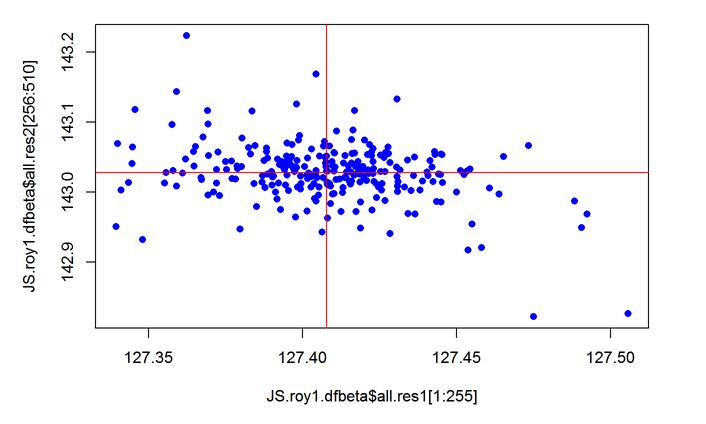
\includegraphics[width=0.7\linewidth]{images/dfbetas-JS-ROY}
	\caption{}
	\label{fig:dfbetas-JS-ROY}
\end{figure}







%---------------------------------------------------------------------------%
%---------------------------------------------------------------------------%


\section{Case Deletion Diagnostics} %1.6

\citet{CPJ} develops \index{case deletion diagnostics} case deletion diagnostics, in particular the equivalent of \index{Cook's distance} Cook's distance, for diagnosing influential observations when estimating the fixed effect parameters and variance components.

\section{Deletion Diagnostics}

Since the pioneering work of Cook in 1977, deletion measures have been applied to many statistical models for identifying influential observations.

Deletion diagnostics provide a means of assessing the influence of an observation (or groups of observations) on inference on the estimated parameters of LME models.

Data from single individuals, or a small group of subjects may influence non-linear mixed effects model selection. Diagnostics routinely applied in model building may identify such individuals, but these methods are not specifically designed for that purpose and are, therefore, not optimal. We describe two likelihood-based diagnostics for identifying individuals that can influence the choice between two competing models.

Case-deletion diagnostics provide a useful tool for identifying influential observations and outliers.

The computation of case deletion diagnostics in the classical model is made simple by the fact that estimates of $\beta$ and $\sigma^2$, which exclude the ith observation, can be computed without re-fitting the model. Such update formulas are available in the mixed model only if you assume that the covariance parameters are not affected by the removal of the observation in question. This is rarely a reasonable assumption.

\subsection*{3. Case Deletion Diagnostics for LME Data: Cooks Distance, DFBetas}
In this section we introduce influence analysis and case deletion diagnosics. A full overview of the topic will be provided although there are specific tools that are particularly useful in the case of MCS problems: specifically the Cook's Distance and the DFBeta.

A discussion of how leave-k-out diagnostics would work in the context of MCS problems is required. There are several scenaros. Suppose we have two methods of measurement X and Y, each with three measurements for a specific case: $(x_1,x_2,x_3,y_1,y_2,y_3)$

\begin{itemize}
	\item Leave One Out - one observation is omitted (e.g. $x_1$)
	\item Leave Pair Out - one pair of observation  is omitted (e.g. $x_1$ and $y_1$)
	\item Leave Case (or Subject) Out - All observations associated with a particular case or subject are omitted. (e.g. $\{x_1,x_2,x_3,y_1,y_2,y_3\}$)
\end{itemize}
Other metrics, such as the likelihood distance, will also be introduced, and revisited in a later section.
%========================================================= %
%- D
\newpage
\subsection*{4. Using DFBETAs to Assess Agreement}
Suppose an LME model was formulated to model agreement for various (i.e. 2 or more) methods of measurement, with replicate measurements. If the methods are to be agreement, the DFBetas for each case would be the same for both methods.\textbf{As such, agreement between any two methods can be determined by a simple scatterplot of the DFBetas. If the points align along the line of equality, then both methods can be said to be in agreement.}

%Cook's Distance can be used to identify and rank cases, in terms of influence.
For the model fitted to the blood data with the lme4 R package, the results tabulated below can be produced. All 85 subjects are ranked by Cook's Distance (with only the top 6 being presented here). The remaining columns are the DFBeta for each of the fixed effects, for each of the 85 subject.
\begin{center}
	\begin{tabular}{|c|c|c|c|c|} \hline
		Subject &    Cook's D  &    methodJ  &   methodR  & methodS \\ \hline \hline
		78 & 0.61557407 & -0.02934556 & -0.03387780 & 0.2954937  \\ \hline
		80 & 0.41590973 & -0.06305026 & -0.06515241 & 0.2123881  \\ \hline
		68 & 0.22536651 & -0.05334867 & -0.05062375 & 0.1555187  \\ \hline
		72 & 0.09348500  & 0.02388626  & 0.02419887 & 0.1617474  \\ \hline
		48 & 0.08706988  & 0.02147541  & 0.03145273 & 0.1581591  \\ \hline
		30 & 0.07118415  & 0.26925807  & 0.26215970 & 0.1581569  \\ \hline
	\end{tabular} 
\end{center}
\newpage
\begin{figure}[h!]
	\centering
	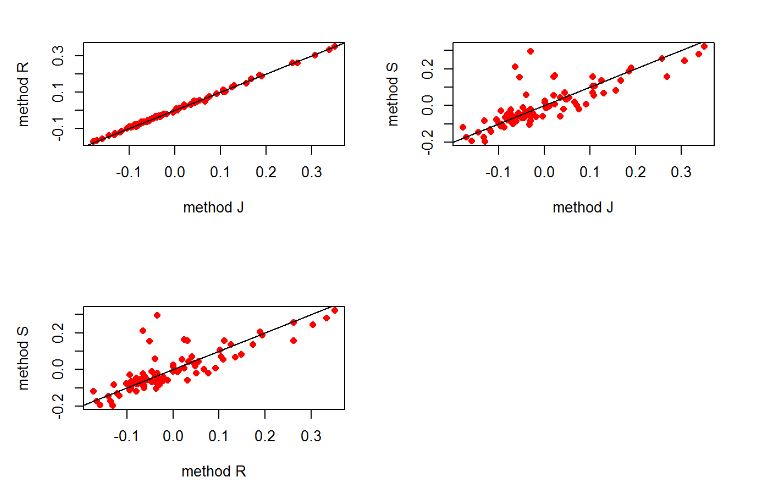
\includegraphics[width=0.9\linewidth]{images/04-DFbetaplots}
	% \caption{}
	% \label{fig:04-DFbetaplots}
\end{figure}

In the first of the three plots (\textit{Top Right}), strong agreement between method J and method R is indicated. The other plots indicate lack of agreement of methods J and R with method S.



If lack of agreement is indicated, a subsequent analysis using a technique proposed by Roy(2009) can be used to identify the specific cause for this lack of agreement (see next section).
\newpage

The Pearson Correlation coefficient of the DFBetas can be used in conjection with this analysis. A high correlation confirms good agreement. No threshold value for agreement is suggested, and analysts are advised to perform model diagnostics regardless of the correlation coeffient. 


The Bonferroni Outlier Test and Cook's Distance values can be used to identify unusual cases, when the relationship between sets of dfbeta is modelled as a (classical) linear model. In this model, the covariates should be homoskedastic. A test for non-constant variance may be used to verify this. These diagnostic procedures are implementable using the \textbf{\textit{car}} R package.

Deming Regression can be used to verify the line of equality. Significance test for Deming regression estimates are not available, but 95\% bootstrap confidence intervals for the slope estimate and intercept estimates can be computed. 


Additionally a mean difference plot can be used to identify outliers. This mean-difference plot differs from the Bland-Altman plot in that the plot is denominated in terms of dfbeta values, and not in measurement units.

If lack of agreement is indicated between methods of measurement, use of Roy's Testing is advised (This is the subject of the next section).
\begin{figure}[h1]
	\centering
	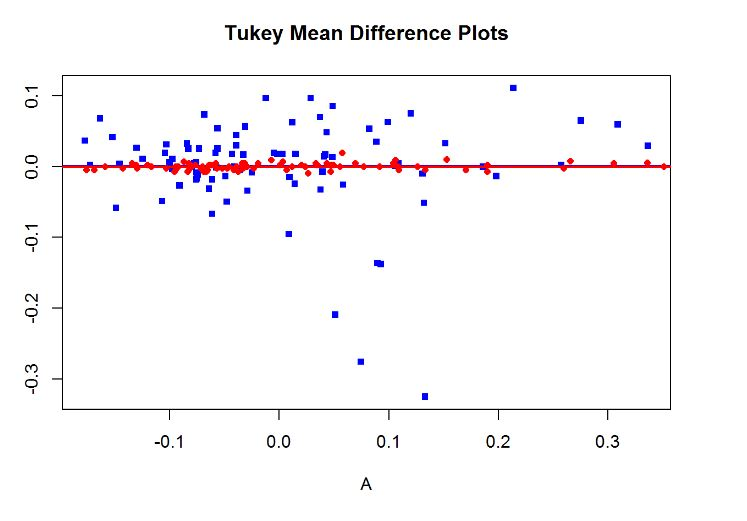
\includegraphics[width=0.7\linewidth]{images/04-TMDplot}
	\caption{}
	\label{fig:04-TMDplot}
\end{figure}
\newpage
%========================================================= %
%% - Part E
\subsection*{5. Using Roy's Test to Identify cause of Lack of agreement}

Barnhart specifies three conditions for method of measurement that are required for two methods of measurement to be considered in agreement.

\begin{itemize}
	\item[(i)] No Significant Inter-method bias
	\item[(ii)] No significant Difference in Within-Subject Variance
	\item[(iii)] No significant Difference in Within-Subject Variance 
\end{itemize}


Roy(2009) demonstrates a LME model specification, and a series of tests that look at each of these agreement criteria individually. If two methods of measuement lack agreement, the specific reason or reasons for this lack of agreement can be identified.


Roy proposes an LME model with Kronecker product covariance structure in a doubly multivariate setup. Response for $i$th subject can be written as
\[ y_i = \beta_0 + \beta_1x_{i1} + \beta_2x_{i2} + b_{1i}z_{i1}  + b_{2i}z_{i2} + \epsilon_i \]
\begin{itemize}
	\item $\beta_1$ and $\beta_2$ are fixed effects corresponding to both methods. ($\beta_0$ is the intercept.)
	\item $b_{1i}$ and $b_{2i}$ are random effects corresponding to both methods.
\end{itemize}

Overall variability between the two methods ($\Omega$) is sum of between-subject ($D$) and within-subject variability ($\Sigma$),
\[
\mbox{Block } \boldsymbol{\Omega}_i = \left[ \begin{array}{cc} d^2_1 & d_{12}\\ d_{12} & d^2_2\\ \end{array} \right]
+ \left[\begin{array}{cc} \sigma^2_1 & \sigma_{12}\\ \sigma_{12} & \sigma^2_2\\ \end{array}\right].
\]
%============================================== %
%- F:
\subsection*{6. Using Roy's Model to Compute LoAs and CR }

In this short section, a demonstration of how Roy's technique can be used to compute two common MCS metrics: Limits of Agreement and the Coefficient of Repeatabilty. While Limits of Agreement are not used in the analysis proposed here, they are ubiquituous in literature, and a demonstration on how to compute them with the Roy Model would assist the adoption of this proposed method.

The coefficient of repeatability is encountered in Gage R \& R analysis. \textit{(A future exploration of how LME models can be used in that field would be of interest. This is something to include in the Conclusions Section).}
%============================================== %
%- G:
\subsection*{7. Model Diagnostics for Roy's Models}

Further to previous work, this section revisits case-deletion and residual diagnostics, and explores how approaches devised by  Galecki \& Burzykowski (2013) can be used to appraise Roy's model. These authors specifically look at Cook's Distances and Likelihood Distances.
For the Roy Model, Cook's Distances may also be generated using the \textbf{\textit{predictmeans}}



\begin{figure}[h!]
	\centering
	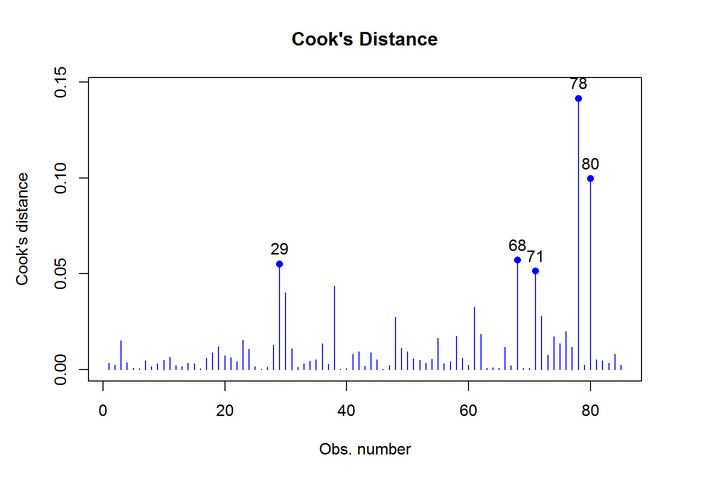
\includegraphics[width=0.7\linewidth]{images/CooksDistancePlot-JS-Roy}
	\caption{}
	\label{fig:CooksDistancePlot-JS-Roy}
\end{figure}

\begin{figure}[h!]
	\centering
	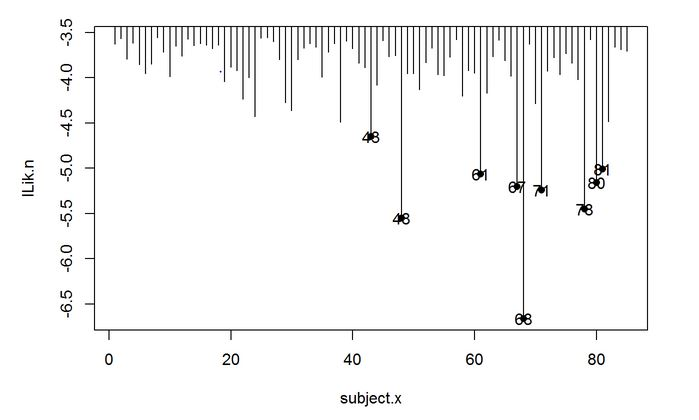
\includegraphics[width=0.7\linewidth]{images/LogLik-JS-Roy}
	\caption{}
	\label{fig:LogLik-JS-Roy}
\end{figure}

As the model is structurally different from the models discussed in the earlier sections, Residual analysis will be briefly revisited.
\begin{figure}[h!]
	\centering
	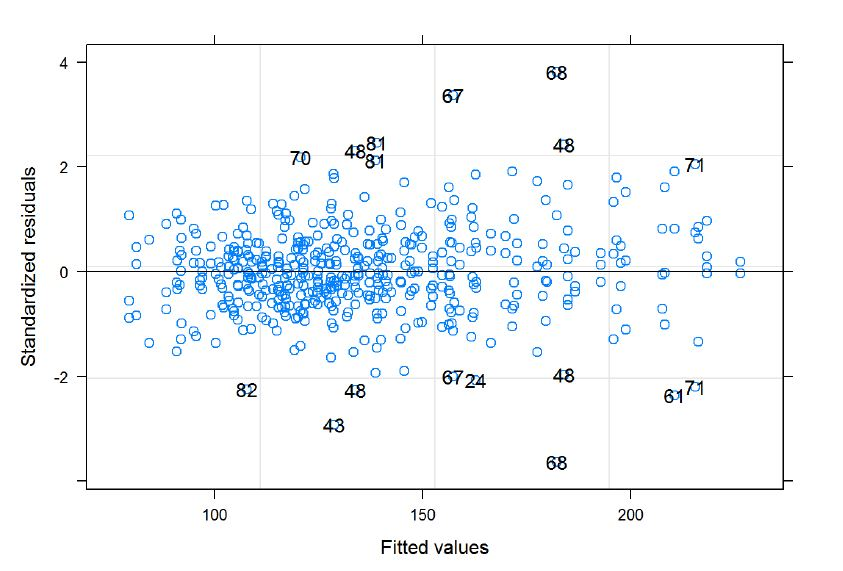
\includegraphics[width=0.7\linewidth]{images/Residuals-JS-Roy}
	\caption{}
	\label{fig:Residuals-JS-Roy}
\end{figure}

\newpage
\subsection*{8. Case Deletion Diagnostics for the Variance Ratios}
%- H Case Deletion Diagnostics 

Schabenberger advises on the use of deletion diagnostics for variance components of an LME model.
Taking the core principals of his methods, and applying them to the Method Comparison problem, case deletion diagnostics are used on the variance components of the Roy model., specifically the ratio of between subject variances and the within subject covariances respecitvely.


\[ \mbox{BSVR} = \frac{\sigma^2_2}{\sigma^2_2} \phantom{makespace}  \mbox{WSVR} = \frac{d^2_2}{d^2_2} \]

These variance ratios are re-computed for each case removed, and may be analysed seperately or jointly for outliers. 

The Grubbs' Test for Outliers is a commonly used technique for assessing outlier in a univariate data set. As there may be several outliers (i.e. influential cases) present, the Grubbs test is not practical. However outlier detection using to Tukey's 
specification for boxplots (i.e. greater than $Q_3 +1.5 IQR$ or less than $Q_1 - 1.5 IQR$), will suffice. Ranking the asbolute values of the standardizaed scores can also can be used to identify influential cases, even if the data is not normally distributed.

Bivariate Analyses may be applied jointly to the both sets of data sets, e.g Mahalanobis distances. The Mahalanobis distance, while not an intuitive measure in the context of the data, can be used to rank highly influential cases. 

%============================================== %
% - I: 
\subsection*{9. Permutation Test, Power Tests and Missing Data }

This section explores topics such as dependent variable simulation and power analysis, introduced by Galecki \& Burzykowski (2013), and implementable with their \textbf{\textit{nlmeU}} \texttt{R} package.
Using the \textbf{\textit{predictmeans}} \texttt{R} package, it is possible to perform permutation t-tests for coefficients of (fixed) effects and permutation F-tests.

The matter of missing data has not been commonly encountered in either Method Comparison Studies or Linear Mixed Effects Modelling. However Roy (2009) deals with the relevant assumptions regrading missing data. Galecki \& Burzykowski (2013) approaches the subject of missing data in LME Modelling. The \textbf{\textit{nlmeU}} package includes the \texttt{patMiss} function, which ``\textit{allows to compactly present pattern of missing data in a given vector/matrix/data
	frame or combination of thereof}".


%================================================%

%-------------------------------------------------------------------------------------------------------------------------------------%
\subsection{Influential Observations : DFBeta and DFBetas}
\section{Measures of Influence} %1.16

The impact of an observation, or a case with multiple obverations, on a regression fitting can be determined by the difference between the estimated regression coefficient of a model with all observations and the estimated coefficient when the particular observation is deleted. The measure DFBETA is the studentized value of this difference.


\section{Overall Influence}
An overall influence statistic measures the change in the objective function being minimized. For example, in
OLS regression, the residual sums of squares serves that purpose. In linear mixed models fit by
\index{maximum likelihood} maximum likelihood (ML) or \index{restricted maximum likelihood} restricted maximum likelihood (REML), an overall influence measure is the \index{likelihood distance} likelihood distance [Cook and Weisberg ].
%============================================================================= %

\section{Effects on fitted and predicted values}
\begin{equation}
	\hat{e_{i}}_{(U)} = y_{i} - x\hat{\beta}_{(U)}
\end{equation}

\section{Case Deletion Diagnostics for Mixed Models}

\citet{Christiansen} notes the case deletion diagnostics techniques have not been applied to linear mixed effects models and seeks to develop methodologies in that respect.

\citet{Christiansen} develops these techniques in the context of REML


\section{Terminology for Case Deletion diagnostics} %1.8

\citet{preisser} describes two type of diagnostics. When the set consists of only one observation, the type is called
'observation-diagnostics'. For multiple observations, Preisser describes the diagnostics as 'cluster-deletion' diagnostics.	\section{Case Deletion Diagnostics}
Case-deletion diagnostics provide a useful tool for identifying influential observations and outliers.

The computation of case deletion diagnostics in the classical model is made simple by the fact that estimates of $\beta$ and $\sigma^2$, which exclude the ith observation, can be computed without re-fitting the model. Such update formulas are available in the mixed model only if you assume that the covariance parameters are not affected by the removal of the observation in question. This is rarely a reasonable assumption.

Linear models for uncorrelated data have well established measures to gauge the influence of one or more
observations on the analysis. For such models, closed-form update expressions allow efficient computations
without refitting the model. 


Since the pioneering work of Cook in 1977, deletion measures have been applied to many statistical models for identifying influential observations. Case-deletion diagnostics provide a useful tool for identifying influential observations and outliers.

The key to making deletion diagnostics useable is the development of efficient computational formulas, allowing one to obtain the \index{case deletion diagnostics} case deletion diagnostics by making use of basic building blocks, computed only once for the full model.

The computation of case deletion diagnostics in the classical model is made simple by the fact that estimates of $\beta$ and $\sigma^2$, which exclude the $i-$th observation, can be computed without re-fitting the model. %\subsection{Terminology for Case Deletion diagnostics} %1.8

\citet{preisser} describes two type of diagnostics. When the set consists of only one observation, the type is called
`\textit{observation-diagnostics}'. For multiple observations, Preisser describes the diagnostics as `\textit{cluster-deletion}' diagnostics. When applied to LME models, such update formulas are available only if one assumes that the covariance parameters are not affected by the removal of the observation in question. However, this is rarely a reasonable assumption.
%--------------------------------------------------------------------------%
\newpage
\section{Case Deletion Diagnostics}

Since the pioneering work of Cook in 1977, deletion measures have been applied to many statistical models for identifying influential observations.

Deletion diagnostics provide a means of assessing the influence of an observation (or groups of observations) on inference on the estimated parameters of LME models.

Data from single individuals, or a small group of subjects may influence non-linear mixed effects model selection. Diagnostics routinely applied in model building may identify such individuals, but these methods are not specifically designed for that purpose and are, therefore, not optimal. We describe two likelihood-based diagnostics for identifying individuals that can influence the choice between two competing models.
Case-deletion diagnostics provide a useful tool for identifying influential observations and outliers.

The computation of case deletion diagnostics in the classical model is made simple by the fact that estimates of $\beta$ and $\sigma^2$, which exclude the ith observation, can be computed without re-fitting the model. Such update formulas are available in the mixed model only if you assume that the covariance parameters are not affected by the removal of the observation in question. This is rarely a reasonable assumption.

\section{Terminology for Case Deletion diagnostics} %1.8

\citet{preisser} describes two type of diagnostics. When the set consists of only one observation, the type is called
'observation-diagnostics'. For multiple observations, Preisser describes the diagnostics as 'cluster-deletion' diagnostics.
\section{influence.ME}

\textit{influence.ME} allows you to compute measures of influential data for mixed effects models generated by lme4.

\textit{influence.ME} provides a collection of tools for detecting influential cases in generalized mixed effects models. It analyses models that were estimated using lme4. The basic rationale behind identifying influential data is that when iteratively single units are omitted from the data, models based on these data should not produce substantially different estimates. 

To standardize the assessment of how influential a (single group of) observation(s) is, several measures of influence are common practice, such as DFBETAS and Cook's Distance. In addition, we provide a measure of percentage change of the fixed point estimates and a simple procedure to detect changing levels of significance.
\newpage

\section{Influence() command}
\texttt{influence()} is the workhorse function of the influence.ME package. Based on a priorly estimated mixed effects regression model (estimated using lme4), the \texttt{influence()} function iteratively modifies the mixed effects model to neutralize the effect a grouped set of data has on the parameters, and which returns returns the fixed parameters of these iteratively modified models. These are used to compute measures of influential data.
%============================================================================= %
\section{Cooks's Distance}
Cook's Distance is a measure indicating to what extent model parameters are influenced by (a set of) influential data on which the model is based. This function computes the Cook's distance based on the information returned by the estex() function.
%============================================================================= %
\chapter{Appendices 1}
\newpage
\subsection{Alternative agreement indices}
As an alternative to limits of agreement, \citet{lin2002} proposes the use of
the mean square deviation is assessing agreement. The mean square
deviation is defined as the expectation of the squared differences
of two readings . The MSD is usually used for the case of two
measurement methods $X$ and $Y$ , each making one measurement for
the same subject, and is given by
\[
MSDxy = E[(x - y)^2]  = (\mu_{x} - \mu_{y})^2 + (\sigma_{x} -
\sigma_{y})^2 + 2\sigma_{x}\sigma_{y}(1-\rho_{xy}).
\]


\citet{Barnhart} advises the use of a predetermined upper limit
for the MSD value, $MSD_{ul}$, to define satisfactory agreement.
However, a satisfactory upper limit may not be properly
determinable, thus creating a drawback to this methodology.


\citet{Barnhart} proposes both the use of the square root of the
MSD or the expected absolute difference (EAD) as an alternative agreement indices. Both of these indices can be interpreted intuitively, being denominated in the same units of measurements as the original
measurements. Also they can be compare to the maximum acceptable
absolute difference between two methods of measurement $d_{0}$.
\[
EAD = E(|x - y|) = \frac{\sum |x_{i}- y_{i}|}{n}
\]

The EAD can be used to supplement the inter-method bias in an
initial comparison study, as the EAD is informative as a measure
of dispersion, is easy to calculate and requires no distributional
assumptions.

\citet{Barnhart} remarks that a comparison of EAD and MSD , using
simulation studies, would be interesting, while further adding
that `It will be of interest to investigate the benefits of these
possible new unscaled agreement indices'. For the Grubbs' `F vs C' and `F vs T' comparisons, the inter-method bias, difference variances, limits of agreement and EADs are shown
in Table 1.5. The corresponding Bland-Altman plots for `F vs C' and `F vs T' comparisons were depicted previously on Figure 1.3. While the inter-method bias for the `F vs T' comparison is smaller, the EAD penalizes the comparison for having a greater variance of differences. Hence the EAD values for both comparisons are much closer.
\begin{table}[ht]
	\begin{center}
		\begin{tabular}{|c|c|c|}
			\hline
			& F vs C & F vs T  \\
			\hline
			Inter-method bias & -0.61 & 0.12 3 \\
			Difference variances & 0.06 & 0.22  \\
			Limits of agreement & (-1.08,	-0.13) & (-0.81,1.04) \\
			EAD & 0.61 & 0.35  \\
			\hline
		\end{tabular}
		\caption{Agreement indices for Grubbs' data comparisons.}
	\end{center}
\end{table}

Further to  \citet{lin2000} and \citet{lin2002}, individual agreement between two measurement methods may be
assessed using the the coverage probability (CP) criteria or the total deviation index (TDI). If $d_{0}$ is predetermined as the maximum acceptable absolute difference between two methods of measurement, the probability that the absolute difference of two measures being less than $d_{0}$ can be computed. This is known as the coverage probability (CP).

\begin{equation}
CP = P(|x_{i} - y_{i}| \leq d_{0})
\end{equation}

If $\pi_{0}$ is set as the predetermined coverage probability, the
boundary under which the proportion of absolute differences is
$\pi_{0}$ may be determined. This boundary is known as the `total
deviation index' (TDI). Hence the TDI is the $100\pi_{0}$
percentile of the absolute difference of paired observations.

\section{LME - Pankaj Choudhury}
Consistent with the conventions of mixed models, \citep{pkc}
formulates the measurement $y_{ij} $from method $i$ on individual
$j$ as follows;
\begin{equation}
	y_{ij} =P_{ij}\theta + W_{ij}v_{i} + X_{ij}b_{j} + Z_{ij}u_{j} +
	\epsilon_{ij},     (j=1,2, i=1,2....n)
\end{equation}
The design matrix $P_{ij}$ , with its associated column vector
$\theta$, specifies the fixed effects common to both methods. The
fixed effect specific to the $j$th method is articulated by the
design matrix $W_{ij}$ and its column vector $v_{i}$. The random
effects common to both methods is specified in the design matrix
$X_{ij}$, with vector $b_{j}$ whereas the random effects specific
to the $i$th subject by the $j$th method is expressed by $Z_{ij}$,
and vector $u_{j}$. Noticeably this notation is not consistent
with that described previously.  The design matrices are specified
so as to includes a fixed intercept for each method, and a random
intercept for each individual. Additional assumptions must also be
specified;
\begin{equation}
	v_{ij} \sim N(0,\Sigma),
\end{equation}
These vectors are assumed to be independent for different $i$s,
and are also mutually independent. All Covariance matrices are
positive definite.  In the above model effects can be classed as
those common to both methods, and those that vary with method.
When considering differences, the effects common to both
effectively cancel each other out. The differences of each pair of
measurements can be specified as following;
\begin{equation}
	d_{ij} = X_{ij}b_{j} + Z_{ij}u_{j} + \epsilon_{ij},     (j=1,2,
	i=1,2....n)
\end{equation}
This formulation has seperate distributional assumption from the
model stated previously.

This agreement covariate $x$ is the key step in how this
methodology assesses agreement.
%%%%%%%%%%%%%%%%%%%%%%%%%%%%%%%%%%%%%%%%%%%%%%%%%%%%%%%%%%%%%%%%%%%%%%%%%%%%%%%%%%%%%%%%%%%%%%%%%%%%%%%5
%----------------------------------------------------------------------------%
\newpage


\section{Model Terms (Roy 2009)}
\begin{itemize}
	\item Let $y_{mir}$ be the response of method $m$ on the $i$th subject
	at the $r-$th replicate.
	\item Let $\boldsymbol{y}_{ir}$ be the $2 \times 1$ vector of measurements
	corresponding to the $i-$th subject at the $r-$th replicate.
	\item Let $\boldsymbol{y}_{i}$ be the $R_i \times 1$ vector of
	measurements corresponding to the $i-$th subject, where $R_i$ is number of replicate measurements taken on item $i$.
	\item Let $\alpha_mi$ be the fixed effect parameter for method for subject $i$.
	\item Formally Roy uses a separate fixed effect parameter to describe the true value $\mu_i$, but later combines it with the other fixed effects when implementing the model.
	\item Let $u_{1i}$ and $u_{2i}$ be the random effects corresponding to methods for item $i$.
	
	\item $\boldsymbol{\epsilon}_{i}$ is a $n_{i}$-dimensional vector
	comprised of residual components. For the blood pressure data $n_{i} = 85$.
	
	\item $\boldsymbol{\beta}$ is the solutions of the means of the two methods. In the LME output, the bias ad corresponding
	t-value and p-values are presented. This is relevant to Roy's first test.\end{itemize}





%------------------------------------------------%
\newpage

\section{Algorithms}
Maximum likelihood estimation is a method of obtaining estimates
of unknown parameters by optimizing a likelihood function. The ML
parameter estimates are the values of the argument that maximise
the likelihood function, i.e. the estimates that make the observed
values of the dependent variable most likely, given the
distributional assumptions

The most common iterative algorithms used for the optimization
problem in the context of LMEs are the EM algoritm, fisher scoring
algorithm and NR algorithm, which [cite:West] commends as the
preferred method.

A mixed model is an extension of the general linear models that
can specify additional random effects terms.

Parameter of the mixed model can be estimated using either ML or
REML, while the AIC and the BIC can be used as measures of
"goodness of fit" for particular models, where smaller values are
considered preferable.

%--------------------------------------------------------------------%


\section{ML v REML}
(\textbf{\emph{Wikipedia}})The restricted (or residual, or reduced) maximum likelihood (REML) approach is a particular form of maximum likelihood estimation which does not base estimates on a maximum likelihood fit of all the information, but instead uses a likelihood function calculated from a transformed set of data, so that nuisance parameters have no effect.

In contrast to the earlier maximum likelihood estimation, REML can produce unbiased estimates of variance and covariance parameters.

%-----------------------------------------------------------------------------------------%
\newpage
\section{ML procedures for LME}

The maximum likelihood procedure of Hartley and Rao yields
simultaneous estimates for both the fixed effects and the random
effect, by maximising the likelihood of $\boldsymbol{y}$ with
respect to each element of $\boldsymbol{\beta}$ and
$\boldsymbol{b}$.

%-----------------------------------------------------------------------------------------%
\newpage
\section{Estimation of random effects}

Estimation of random effects for LME models in the NLME package is accomplished through use
of both EM (Expectation-Maximization) algorithms and Newton-Raphson algorithms.
\begin{itemize}
	\item EM iterations bring estimates of the parameters into the region of the optimum very quickly, but
	convergence to the optimum is slow when near the optimum.
	\item Newton-Raphson iterations are computationally intensive and can be unstable when far from the
	optimum. However, close to the optimum they converge quickly.
	\item The LME function implements a hybrid approach, using 25 EM iterations to quickly get near the
	optimum, then switching to Newton-Raphson iterations to quickly converge to the optimum. \item If
	convergence problems occur, the ``control� argument in LME can be used to change the way the
	model arrives at the optimum.
\end{itemize}







\bibliographystyle{chicago}
\bibliography{DB-txfrbib}
\end{document}

%---------------------------------------------------------------------------------------------------%


